% Options for packages loaded elsewhere
\PassOptionsToPackage{unicode}{hyperref}
\PassOptionsToPackage{hyphens}{url}
%
\documentclass[
  doc,floatsintext]{apa6}
\usepackage{amsmath,amssymb}
\usepackage{iftex}
\ifPDFTeX
  \usepackage[T1]{fontenc}
  \usepackage[utf8]{inputenc}
  \usepackage{textcomp} % provide euro and other symbols
\else % if luatex or xetex
  \usepackage{unicode-math} % this also loads fontspec
  \defaultfontfeatures{Scale=MatchLowercase}
  \defaultfontfeatures[\rmfamily]{Ligatures=TeX,Scale=1}
\fi
\usepackage{lmodern}
\ifPDFTeX\else
  % xetex/luatex font selection
\fi
% Use upquote if available, for straight quotes in verbatim environments
\IfFileExists{upquote.sty}{\usepackage{upquote}}{}
\IfFileExists{microtype.sty}{% use microtype if available
  \usepackage[]{microtype}
  \UseMicrotypeSet[protrusion]{basicmath} % disable protrusion for tt fonts
}{}
\makeatletter
\@ifundefined{KOMAClassName}{% if non-KOMA class
  \IfFileExists{parskip.sty}{%
    \usepackage{parskip}
  }{% else
    \setlength{\parindent}{0pt}
    \setlength{\parskip}{6pt plus 2pt minus 1pt}}
}{% if KOMA class
  \KOMAoptions{parskip=half}}
\makeatother
\usepackage{xcolor}
\usepackage{graphicx}
\makeatletter
\def\maxwidth{\ifdim\Gin@nat@width>\linewidth\linewidth\else\Gin@nat@width\fi}
\def\maxheight{\ifdim\Gin@nat@height>\textheight\textheight\else\Gin@nat@height\fi}
\makeatother
% Scale images if necessary, so that they will not overflow the page
% margins by default, and it is still possible to overwrite the defaults
% using explicit options in \includegraphics[width, height, ...]{}
\setkeys{Gin}{width=\maxwidth,height=\maxheight,keepaspectratio}
% Set default figure placement to htbp
\makeatletter
\def\fps@figure{htbp}
\makeatother
\setlength{\emergencystretch}{3em} % prevent overfull lines
\providecommand{\tightlist}{%
  \setlength{\itemsep}{0pt}\setlength{\parskip}{0pt}}
\setcounter{secnumdepth}{-\maxdimen} % remove section numbering
% Make \paragraph and \subparagraph free-standing
\makeatletter
\ifx\paragraph\undefined\else
  \let\oldparagraph\paragraph
  \renewcommand{\paragraph}{
    \@ifstar
      \xxxParagraphStar
      \xxxParagraphNoStar
  }
  \newcommand{\xxxParagraphStar}[1]{\oldparagraph*{#1}\mbox{}}
  \newcommand{\xxxParagraphNoStar}[1]{\oldparagraph{#1}\mbox{}}
\fi
\ifx\subparagraph\undefined\else
  \let\oldsubparagraph\subparagraph
  \renewcommand{\subparagraph}{
    \@ifstar
      \xxxSubParagraphStar
      \xxxSubParagraphNoStar
  }
  \newcommand{\xxxSubParagraphStar}[1]{\oldsubparagraph*{#1}\mbox{}}
  \newcommand{\xxxSubParagraphNoStar}[1]{\oldsubparagraph{#1}\mbox{}}
\fi
\makeatother
% definitions for citeproc citations
\NewDocumentCommand\citeproctext{}{}
\NewDocumentCommand\citeproc{mm}{%
  \begingroup\def\citeproctext{#2}\cite{#1}\endgroup}
\makeatletter
 % allow citations to break across lines
 \let\@cite@ofmt\@firstofone
 % avoid brackets around text for \cite:
 \def\@biblabel#1{}
 \def\@cite#1#2{{#1\if@tempswa , #2\fi}}
\makeatother
\newlength{\cslhangindent}
\setlength{\cslhangindent}{1.5em}
\newlength{\csllabelwidth}
\setlength{\csllabelwidth}{3em}
\newenvironment{CSLReferences}[2] % #1 hanging-indent, #2 entry-spacing
 {\begin{list}{}{%
  \setlength{\itemindent}{0pt}
  \setlength{\leftmargin}{0pt}
  \setlength{\parsep}{0pt}
  % turn on hanging indent if param 1 is 1
  \ifodd #1
   \setlength{\leftmargin}{\cslhangindent}
   \setlength{\itemindent}{-1\cslhangindent}
  \fi
  % set entry spacing
  \setlength{\itemsep}{#2\baselineskip}}}
 {\end{list}}
\usepackage{calc}
\newcommand{\CSLBlock}[1]{\hfill\break\parbox[t]{\linewidth}{\strut\ignorespaces#1\strut}}
\newcommand{\CSLLeftMargin}[1]{\parbox[t]{\csllabelwidth}{\strut#1\strut}}
\newcommand{\CSLRightInline}[1]{\parbox[t]{\linewidth - \csllabelwidth}{\strut#1\strut}}
\newcommand{\CSLIndent}[1]{\hspace{\cslhangindent}#1}
\ifLuaTeX
\usepackage[bidi=basic]{babel}
\else
\usepackage[bidi=default]{babel}
\fi
\babelprovide[main,import]{english}
% get rid of language-specific shorthands (see #6817):
\let\LanguageShortHands\languageshorthands
\def\languageshorthands#1{}
% Manuscript styling
\usepackage{upgreek}
\captionsetup{font=singlespacing,justification=justified}

% Table formatting
\usepackage{longtable}
\usepackage{lscape}
% \usepackage[counterclockwise]{rotating}   % Landscape page setup for large tables
\usepackage{multirow}		% Table styling
\usepackage{tabularx}		% Control Column width
\usepackage[flushleft]{threeparttable}	% Allows for three part tables with a specified notes section
\usepackage{threeparttablex}            % Lets threeparttable work with longtable

% Create new environments so endfloat can handle them
% \newenvironment{ltable}
%   {\begin{landscape}\centering\begin{threeparttable}}
%   {\end{threeparttable}\end{landscape}}
\newenvironment{lltable}{\begin{landscape}\centering\begin{ThreePartTable}}{\end{ThreePartTable}\end{landscape}}

% Enables adjusting longtable caption width to table width
% Solution found at http://golatex.de/longtable-mit-caption-so-breit-wie-die-tabelle-t15767.html
\makeatletter
\newcommand\LastLTentrywidth{1em}
\newlength\longtablewidth
\setlength{\longtablewidth}{1in}
\newcommand{\getlongtablewidth}{\begingroup \ifcsname LT@\roman{LT@tables}\endcsname \global\longtablewidth=0pt \renewcommand{\LT@entry}[2]{\global\advance\longtablewidth by ##2\relax\gdef\LastLTentrywidth{##2}}\@nameuse{LT@\roman{LT@tables}} \fi \endgroup}

% \setlength{\parindent}{0.5in}
% \setlength{\parskip}{0pt plus 0pt minus 0pt}

% Overwrite redefinition of paragraph and subparagraph by the default LaTeX template
% See https://github.com/crsh/papaja/issues/292
\makeatletter
\renewcommand{\paragraph}{\@startsection{paragraph}{4}{\parindent}%
  {0\baselineskip \@plus 0.2ex \@minus 0.2ex}%
  {-1em}%
  {\normalfont\normalsize\bfseries\itshape\typesectitle}}

\renewcommand{\subparagraph}[1]{\@startsection{subparagraph}{5}{1em}%
  {0\baselineskip \@plus 0.2ex \@minus 0.2ex}%
  {-\z@\relax}%
  {\normalfont\normalsize\itshape\hspace{\parindent}{#1}\textit{\addperi}}{\relax}}
\makeatother

\makeatletter
\usepackage{etoolbox}
\patchcmd{\maketitle}
  {\section{\normalfont\normalsize\abstractname}}
  {\section*{\normalfont\normalsize\abstractname}}
  {}{\typeout{Failed to patch abstract.}}
\patchcmd{\maketitle}
  {\section{\protect\normalfont{\@title}}}
  {\section*{\protect\normalfont{\@title}}}
  {}{\typeout{Failed to patch title.}}
\makeatother

\usepackage{xpatch}
\makeatletter
\xapptocmd\appendix
  {\xapptocmd\section
    {\addcontentsline{toc}{section}{\appendixname\ifoneappendix\else~\theappendix\fi: #1}}
    {}{\InnerPatchFailed}%
  }
{}{\PatchFailed}
\makeatother
\keywords{Trust in science; conspiracy theories; conspiracy thinking; science knowledge.}
\usepackage{csquotes}
\usepackage{placeins} 

\ifLuaTeX
  \usepackage{selnolig}  % disable illegal ligatures
\fi
\usepackage{bookmark}
\IfFileExists{xurl.sty}{\usepackage{xurl}}{} % add URL line breaks if available
\urlstyle{same}
\hypersetup{
  pdftitle={Quasi-universal acceptance of basic science in the US},
  pdflang={en-EN},
  pdfkeywords={Trust in science; conspiracy theories; conspiracy thinking; science knowledge.},
  hidelinks,
  pdfcreator={LaTeX via pandoc}}

\title{Quasi-universal acceptance of basic science in the US}
\author{\textsuperscript{}}
\date{}


\shorttitle{Does anyone mistrust basic science?}

\affiliation{\vspace{0.5cm}\textsuperscript{} }

\abstract{%
Substantial minorities of the population report a low degree of trust in science, or endorse conspiracy theories that violate basic scientific knowledge. This might indicate a wholesale rejection of science. In four studies, we asked 782 US participants questions about trust in science, conspiracy beliefs, and basic science (e.g.~the relative size of electrons and atoms). Participants were provided with the scientifically consensual answer to the basic science questions, and asked whether they accept it. Acceptance of the scientific consensus was very high in the sample as a whole (95.1\%), but also in every sub-sample (e.g., no trust in science: 87.3\%; complete endorsement of flat Earth theory: 87.2\%). This quasi-universal acceptance of basic science suggests that people are motivated to reject specific scientific beliefs, and not science as a whole. This could be leveraged in science communication.
}



\begin{document}
\maketitle

\section{Introduction}\label{introduction}

Trust in science is related to many desirable outcomes, from acceptance of anthropogenic climate change (Cologna \& Siegrist, 2020) or vaccination (Lindholt, Jørgensen, Bor, \& Petersen, 2021; Sturgis, Brunton-Smith, \& Jackson, 2021) to following recommendations during COVID (Algan, Cohen, Davoine, Foucault, \& Stantcheva, 2021, which suggests that trust in science was the most important predictor of these behaviors).

Although recent global evidence suggests that trust in science is moderately high (Cologna et al., 2024), it is far from being at ceiling. Large-scale polls have shown that people who report a high degree of trust in science are a minority in most countries, and they are outnumbered by people who have low trust in science in many areas, e.g., most of Africa and significant parts of Asia (Wellcome Global Monitor, 2018, 2020). Moreover, trust in science has recently been declining in some countries Funk \& Kennedy (2020), including the US (Brian \& Tyson, 2023), where it is also increasingly polarizing (Gauchat, 2012; Krause, Brossard, Scheufele, Xenos, \& Franke, 2019; Li \& Qian, 2022).

Besides low answers on general trust in science questions, another indicator of distrust in science is the belief in conspiracy theories that question the scientific consensus on issues such as vaccination, climate change, and even the shape of the Earth. Conspiracy theories--in the realm of science or elsewhere--typically accuse a small group of powerful people to pursue nefarious goals in secrecy (Douglas et al., 2019; Mede \& Schäfer, 2020). Some of these conspiracy theories are widespread (Rutjens \& Većkalov, 2022). In 2023, a survey in eight different countries found that up to 24\% of respondents agreed that ``climate change is a hoax and scientists touting its existence are lying'' (Stockemer \& Bordeleau, 2024). Similarly, in 2021, 40\% of Americans believed that ``the dangers of genetically-modified foods are being hidden from the public'' (down from 45\% in 2020, Uscinski et al., 2022). People who hold such views not only reject the relevant scientifically consensual facts, but also tend to believe in other conspiracy theories (Hornsey, Harris, \& Fielding, 2018b, 2018a; Lewandowsky, Gignac, \& Oberauer, 2013) and tend to say that they distrust science more generally (Stockemer \& Bordeleau, 2024; Vranic, Hromatko, \& Tonković, 2022). Despite these correlations, the causal relationship between declaring general distrust in science and believing in one or several anti-science conspiracy theories is not clear. Although conspiracy thinking been identified as a ``root cause'' of anti-science attitudes (Hornsey \& Fielding, 2017) in the past, these claims rest largely on observational data.

What does this apparent lack of trust in science actually entail? Do people who say they do not trust science, or who believe in conspiracy theories at odds with well-established science, reject most of science? Or, on the contrary, do they object to a few specific facets of science, while still accepting the overwhelming majority of basic science?

A common conception of trust is a willingness to be vulnerable to another party, whether an individual, a group, or an institution (Mayer, Davis, \& Schoorman, 1995; Rousseau, Sitkin, Burt, \& Camerer, 1998). Accordingly, trust in science has been defined as ``one's willingness to rely on science and scientists (as representatives of the system) despite having a bounded understanding of science'' (Wintterlin et al., 2022, p. 2). Past research has disentangled this general concept of trust in science in various ways. Some research has identified different components of trust, the number of which varies, but which generally cover an epistemological and ethical dimension (Intemann, 2023; Wilholt, 2013). For example, Hendriks, Kienhues, and Bromme (2015) suggest distinguishing between expertise/competence, integrity, and benevolence, while Besley, Lee, and Pressgrove (2021) add openness. Other research has highlighted differences in trust between scientific disciplines (Altenmüller, Wingen, \& Schulte, 2024; Gauchat \& Andrews, 2018; Gligorić, Kleef, \& Rutjens, 2024). However, little research has assessed trust in specific scientific findings, besides contentious topics such as vaccines (e.g. Hornsey et al., 2018b), climate change (e.g. Stockemer \& Bordeleau, 2024), evolution (e.g. Nadelson \& Hardy, 2015), genetically modified organisms (GMOs) (e.g. Fernbach, Light, Scott, Inbar, \& Rozin, 2019), or a combinations of such topics (see e.g Lewandowsky et al., 2013). To the best of our knowledge, no research has investigated the extent to which people trust basic science facts (e.g.~electrons are smaller than atoms). An extensive literature on science literacy has assessed whether people know such facts (National Academies of Sciences, Engineering, and Medicine, 2016), but not whether they accept the facts once presented to them.

Why does it matter whether trust in science in general is or is not related to trust in scientific findings? First, this question has theoretical implications. According to the most prominent explanation of (dis)trust in science--the deficit model--science knowledge is the main driver of attitudes towards science in general. A prediction of this model is that average trust in science on specific facts should be strongly associated with general trust in science. By contrast, a disconnect between the two would be in line with motivated reasoning accounts of trust in science. According to these accounts, science rejection serves to maintain coherence with other beliefs or behaviors (Hornsey, 2020; Lewandowsky \& Oberauer, 2016). For example, someone might say they don't trust science in general because they are skeptical towards vaccines, not because they actually distrust most of science. A prediction of the motivated reasoning account is that general trust in science should be strongly correlated with conspiracy beliefs. Second, the present question has practical implications: Many communication attempts leverage the scientific consensus (e.g.~on vaccination, climate change, etc., for review, see Van Stekelenburg, Schaap, Veling, Van 'T Riet, \& Buijzen, 2022; see also Većkalov et al., 2024). These attempts are more likely to be successful if everyone trusts basic science than if some people reject science wholesale.

\subsection{The present studies}\label{the-present-studies}

In a series of four pre-registered online studies (total n = 782), we asked US participants questions about well-established, consensual scientific facts. For each question, we asked participants what they thought the correct answer was (testing their knowledge of science), we informed them of the scientifically accepted answer, and asked them whether they accepted it (measuring their trust in basic science). We also measured participants' trust in science using standard measures, as well as their beliefs in various conspiracy theories and their tendency to engage in conspiratorial thinking. The four studies, including materials, hypotheses, and analyses, were pre-registered and all materials and data are accessible via the Open Science Framework (\url{https://osf.io/8utsj/?view_only=364478f01fc548d0a42b9962918d871d}). The differences between the four studies are summarized presently, and the methods are detailed below.

\subsubsection{Materials}\label{materials}

In Study 1 (data collected on March 5, 2024), we used questions drawn from questionnaires of scientific knowledge (e.g.~``Are electrons smaller, larger, or the same size as atoms? {[}Smaller; Same size; Larger{]}''), supplemented by a `trick' question (``Where do trees mainly draw the materials with which they create their mass? {[}Earth; Water; Air{]}''; correct answer: Air). In Studies 2 (data collected on April 3, 2024) and 3 (data collected on April 22, 2024), this last question was removed. The scientific facts used in Studies 1 to 3 represent long-established and basic knowledge. In Study 4 (data collected on August 13, 2024) we used more recent, much less basic scientific discoveries (e.g.~``What is the electric charge of the Higgs Boson, as established in 2012? {[}1.602176634 × 10-19; 0; 3.2×10-19C{]}''; correct answer: 0, i.e.~electrically neutral).

\subsubsection{Presentation of the scientific consensus}\label{presentation-of-the-scientific-consensus}

In Study 1, we simply told participants that they would be provided with the scientifically consensual answer. However, for participants to accept this answer, they must not only trust science, but also trust that we are presenting them with the actual scientifically consensual answer. To remove this issue, in Studies 2 to 3, we presented participants with a short explanation of the correct answer, as well as links to three sources per answer (e.g.~Wikipedia, National Geographic or NASA). In Study 4, as the topics were more complex, we did not provide an explanation, but still provided two sources per answer.

\subsubsection{Measure of acceptance of the scientific consensus}\label{measure-of-acceptance-of-the-scientific-consensus}

In Study 1, we simply looked at whether participants accept the scientifically consensual answer or not. In the subsequent studies, we asked participants to explain cases in which they disagreed with the scientific consensus. This revealed that a number of participants had made a mistake (misunderstanding, selecting the wrong answer). As a result, in Studies 3 and 4, participants who have indicated that they rejected the scientifically consensual answer were offered the option to revise their answer, or to keep rejecting it.

\subsubsection{Additional questions}\label{additional-questions}

In Studies 3 and 4, we attempted to understand how some people who say they do not trust science still accept scientifically consensual answers, by asking them whether they accepted the answers on the basis of trust in science or because they had independently verified them.

\subsubsection{Samples}\label{samples}

Studies 1 and 2 were conducted on the standard sample of US participants recruited on the platform Prolific Academic. In order to increase the share of participants with low trust in science, and who endorse conspiracy theories, Studies 3 and 4 used the same platform, but only recruited participants who had declared previously being skeptical of vaccination.

\subsubsection{Hypotheses}\label{hypotheses}

The main goal of the present studies is descriptive: to find out whether participants who report not trusting science, or who believe in conspiracy theories, still accept most well-established scientific facts. However, based on our literature review, we also tested two directional hypotheses (pre-registered as research questions in the Study 1):

\textbf{H1: Higher trust in science is associated with more science knowledge and more acceptance of the scientific consensus}

\textbf{H2: Higher conspiracy thinking/belief is associated with less science knowledge and less acceptance of the scientific consensus}

\section{Methods}\label{methods}

\subsection{Deviations from preregistration}\label{deviations-from-preregistration}

For Study 2, we restricted our main hypotheses about acceptance to cases in which participants initially provided a wrong answer. However, this meant the more participants had initially provided correct answers, the fewer opportunities they had for accepting correct answers. We provide results on these conditional correlations--for Study 2 and for all other studies--in the ESM, section \ref{exp1} to \ref{exp4} \footnote{Only in Study 4 do we find evidence that changing one's mind towards the scientific consensus is associated with (more) trust in science (Studies 1: r = 0.06, p = 0.387; 2: r = 0.16, p = 0.051; 3: r = 0.04, p = 0.619; 4: r = 0.15, p = 0.037) and only in Study 2 evidence that it is associated with (less) conspiracy beliefs and (less) conspiracy thinking (Studies 1: r = -0.14, p = 0.061; 2: r = -0.22, p = 0.006; 3: r = -0.04, p = 0.631; 4: r = -0.05, p = 0.455).}. However, for the analysis presented here, we proceeded as preregistered for all other studies, by reporting unconditional correlations between acceptance and trust in science, or, respectively, conspiracy belief.

\subsection{Procedure}\label{procedure}

After providing their consent to participate in the study, participants were given an attention check ``While watching the television, have you ever had a fatal heart attack?'' {[}1-6; 1 = Never, 6 = Often{]}. All participants who did not answer ``1 = Never'' were excluded. Participants then read the following instructions:``We will ask you 10 questions about science. After each question, we will provide you with the scientifically consensual answer and ask whether you accept it.'' Next, participants answered a set of 10 basic science questions in random order. After each question, participants were presented with an answer reflecting the scientific consensus, and asked whether they accepted it. In Studies 2 and 3, participants additionally saw a short explanation, partly based on explanations generated by ChatGPT, and three links to authoritative sources supporting the answer. In Study 4, we provided only two links and no explanation. Participants then answered questions on conspiracy thinking, conspiracy beliefs, and trust in science.

In Studies 2, 3, and 4, we presented participants with open-ended questions so they could explain their rejection of the scientific consensus. In Studies 3 and 4, we additionally gave participants the option to change their answer and accept the scientific consensus. Finally, at the end of Studies 3 and 4, we asked participants: ``For the questions in which you agreed with the scientific consensus, would you say that\ldots?'' The answer options were: (i) ``You mostly agree with the consensus because, on that question, you trust scientists'', (ii) ``You mostly agree with the consensus because you have been able to independently verify it'', and (iii) ``Other'', with a text box for participants to explain. Participants who selected ``You mostly agree with the consensus because you have been able to independently verify it'', were asked the open-ended follow-up question: ``Could you please tell us how you independently verified the information?''.

\subsection{Participants}\label{participants}

After removing failed attention checks, the total sample size was 782 (194 in Study 1, six failed attention checks; 190 in Study 2, 11 failed attention checks; 200 in Study 3, no failed attention checks; 198 in Study 4, two failed attention checks) participants in the US, recruited through Prolific. Details and demographics can be found in the online supplemental material. While samples for Studies 1 and 2 were convenience samples, Studies 3 and 4 were conducted on a sample holding vaccine-skeptic beliefs. Prolific allows selecting participants based on their answers to a range of questions. We picked three of these questions and only recruited participants who met our criteria for each of them:

\begin{enumerate}
\def\labelenumi{\arabic{enumi}.}
\tightlist
\item
  ``Please describe your attitudes towards the COVID-19 (Coronavirus) vaccines: {[}For (I feel positively about the vaccines); Against (I feel negatively about the vaccines); Neutral (I don't have strong opinions either way); Prefer not to say{]}''. We selected participants who answered ``Against''.
\item
  ``Have you received a coronavirus (COVID-19) vaccination? {[}Yes (at least one dose); No; Prefer not to answer{]}''. We select only people who answered ``No''.
\item
  ``On a scale from 1-7, please rate to what extent you agree with the following statement: I believe that scheduled immunizations are safe for children. {[}1 (totally disagree); 2 (disagree); 3 (somewhat disagree); 4 (neither agree nor disagree); 5 (somewhat agree); 6 (agree); 7 (totally agree); rather not say{]}''. We select only people who answered ``1'', ``2'', or ``3''.
\end{enumerate}

\subsection{Materials}\label{materials-1}

\subsubsection{Scientific facts}\label{scientific-facts}

Studies 1 to 3 used 10 facts drawn from widely used questionnaires about science knowledge (Allum, Sturgis, Tabourazi, \& Brunton-Smith, 2008; Durant, Evans, \& Thomas, 1989; Miller, 1998) sometimes referred to as the ``Oxford scale'' (Gauchat, 2011). A `trick' question was added in Study 1 and removed as its wording proved unclear. Study 4 used 10 more recent scientific discoveries. Table \ref{tab:knowledge} shows all questions and their answer options.

\begingroup\fontsize{8}{10}\selectfont

\begin{longtable}[t]{>{\raggedleft\arraybackslash}p{2em}>{\raggedright\arraybackslash}p{22em}>{\raggedright\arraybackslash}p{22em}}
\caption{\label{tab:knowledge}Science knowledge items}\\
\toprule
 & Study 1-3 & Study 4\\
\midrule
1 & Do antibiotics kill viruses as well as bacteria? [Yes, both; No, only viruses; No, only bacteria] & For which disease is the drug bedaquiline, developed in 2007, a treatment? [Tetanus; Tuberculosis; Malaria]\\
2 & Are electrons smaller, larger, or the same size as atoms? [Smaller; Same size; Larger] & What is the maximum speed a proton can attain in the largest particle collider as to 2015? [90\% of the speed of light; 99\% of the speed of light; the speed of light]\\
3 & Have the continents on Earth been moving for millions of years or have they always been where they are now? [They have been moving; They have always been where they are now] & Kepler-452b is an exoplanet revolving around the star Kepler-452. How far away from the star is it, as established by astronomers in 2015? [97 million mi; 1,2 million mi; 1254 million mi]\\
4 & What decides whether a baby is a boy or a girl ? Is it the father's genes, the mother's genes, or both? [The mother's genes; the father's genes; both] & Using bomb-pusle dating with carbon 14, what is the age of the oldest known vertebrate, as established in 2016? [138 years; 205 years;  392 years]\\
5 & Do lasers work by focusing sound waves? [Yes; No] & How many more glial cells are there in the brain in comparison with neurons, as established in 2016? [The same amount; Twice as many; Ten times as many]\\
\addlinespace
6 & How long does it take for Earth to go around the sun: one day, one month, or one year? [One day; One month; One year] & As predicted by the general theory of relativity, how many times would the Earth keep orbiting if the Sun disappeared, as established in 2012? [47 seconds; 8 minutes;  2 hours]\\
7 & Are diamonds made of carbon? [Yes; No] & What is the electric charge of the Higgs Boson, as established in 2012? [1.602176634 x 10-19; 0; 3.2x10-19C]\\
8 & Which travels faster : light or sound? [Light; Sound] & What is the age of the oldest materials formed on Earth, as established in 2020? [Less than 4.6 Ga; Around 4.6 Ga; More than 4.6 Ga]\\
9 & Is common table salt made of calcium carbonate? [Yes; No] & With the best current cloning techniques, what is the average success rate when operated on mice, as of 2010? [2,7\%; 9,4\%; 17,2\%]\\
10 & Is water made of molecules containing one oxygen and two hydrogen atoms? [Yes; No] & What was the strength of the Earth magnetic field 3.7 billion years ago, as discovered this year? [15 microtesla; 30 microtesla; 45 microtesla]\\
\addlinespace
11 & *Where do trees mainly draw the materials with which they create their mass? [Earth; Water; Air] & \\
\bottomrule
\multicolumn{3}{l}{\rule{0pt}{1em}\textsuperscript{*} Only used in Study 1}\\
\end{longtable}
\endgroup{}

\subsubsection{Conspiracy beliefs}\label{conspiracy-beliefs}

We selected 10 science/health related conspiracy theories from the Belief in Conspiracy Theory Inventory (BCTI) (Pennycook, Binnendyk, \& Rand, 2022) (Table \ref{tab:conspiracy}). Participants were asked: ``Below is a list of events for which the official version has been disputed. For each event, we would like you to indicate to what extent you believe the cover-up version of events is true or false. {[}1-9; labels: 1 - completely false, 5 - unsure, 9 - completely true{]}''.

\subsubsection{Conspiracy thinking}\label{conspiracy-thinking}

For all results presented here, we used the four-item conspiracy mentality questionnaire (CMQ) (Bruder, Haffke, Neave, Nouripanah, \& Imhoff, 2013). We also assessed the single item conspiracy beliefs scale (SICBS) (Lantian, Muller, Nurra, \& Douglas, 2016). Details and comparisons between the scales can be found in the ESM, sections \ref{exp1} to \ref{exp4}.

\begingroup\fontsize{8}{10}\selectfont

\begin{ThreePartTable}
\begin{TableNotes}[para]
\item \textit{Note: } 
\item Participants were asked to rate their belief in the conspiracy on a scale from 1 to 9, with the labels: `1 - completely false, 5 - unsure, 9 - completely true`.
\end{TableNotes}
\begin{longtable}[t]{>{\raggedleft\arraybackslash}p{3em}>{\raggedright\arraybackslash}p{40em}}
\caption{\label{tab:conspiracy}Conspiracy items}\\
\toprule
1 & The Apollo moon landings never happened and were staged in a Hollywood film studio.\\
2 & A cure for cancer was discovered years ago, but this has been suppressed by the pharmaceutical industry and the U.S. Food and Drug Administration (FDA).\\
3 & The spread of certain viruses and/or diseases is the result of the deliberate, concealed efforts of vested interests.\\
4 & The claim that the climate is changing due to emissions from fossil fuels is a hoax perpetrated by corrupt scientists who want to spend more taxpayer money on climate research.\\
5 & The Earth is flat (not spherical) and this fact has been covered up by scientists and vested interests.\\
\addlinespace
6 & There is a causal link between vaccination and autism that has been covered up by the pharmaceutical industry.\\
7 & In the 1950s and 1960s more than 100 million Americans received a polio vaccine contaminated with a potentially cancer-causing virus.\\
8 & Proof of alien contact is being concealed from the public.\\
9 & Hydroxychloroquine has been demonstrated to be a safe and effective treatment of COVID and this information is being suppressed.\\
10 & Dinosaurs never existed, evolution is not real, and scientists have been faking the fossil record.\\
\bottomrule
\insertTableNotes
\end{longtable}
\end{ThreePartTable}
\endgroup{}

\subsubsection{Trust in science}\label{trust-in-science}

In all analyses reported in the main paper, we measure trust in science via a question selected from the Wellcome Global Monitor surveys (Wellcome Global Monitor, 2018, 2020): ``In general, would you say that you trust science a lot, some, not much, or not at all? {[}1 = Not at all, 2 = Not much, 3 = Some, 4 = A lot{]}''. We chose this question as it seemed to be the most general one. In the ESM (sections \ref{exp1} to \ref{exp4}), we additionally report results for two alternative measures of trust included in our studies: Another from the WGM surveys (``How much do you trust scientists in this country? Do you trust them a lot, some, not much, or not at all? {[}1 = Not at all, 2 = Not much, 3 = Some, 4 = A lot{]}''), and one from the Pew Research Center (e.g. Funk, Johnson, \& Hefferon, 2019) (``How much confidence do you have in scientists to act in the best interests of the public? {[}1-5; 1 = No confidence at all, 5 = A great deal of confidence{]}''), the latter having been used in a recent international study on trust in science (Cologna et al., 2024). We selected these items so that we could compare the answers in our sample to global survey results. We find that all three items are highly correlated throughout all studies, and that our results reported here generally replicate when using either of the alternatives measures\footnote{With two exceptions: In Study 3, we find no correlation between acceptance and the Pew question; In Study 4, we find a correlation between knowledge and both alternative trust measures, but not with our main measure; see ESM, sections \ref{exp3} and \ref{exp4}} (see ESM).

\section{Results}\label{results}



\begin{figure}
\centering
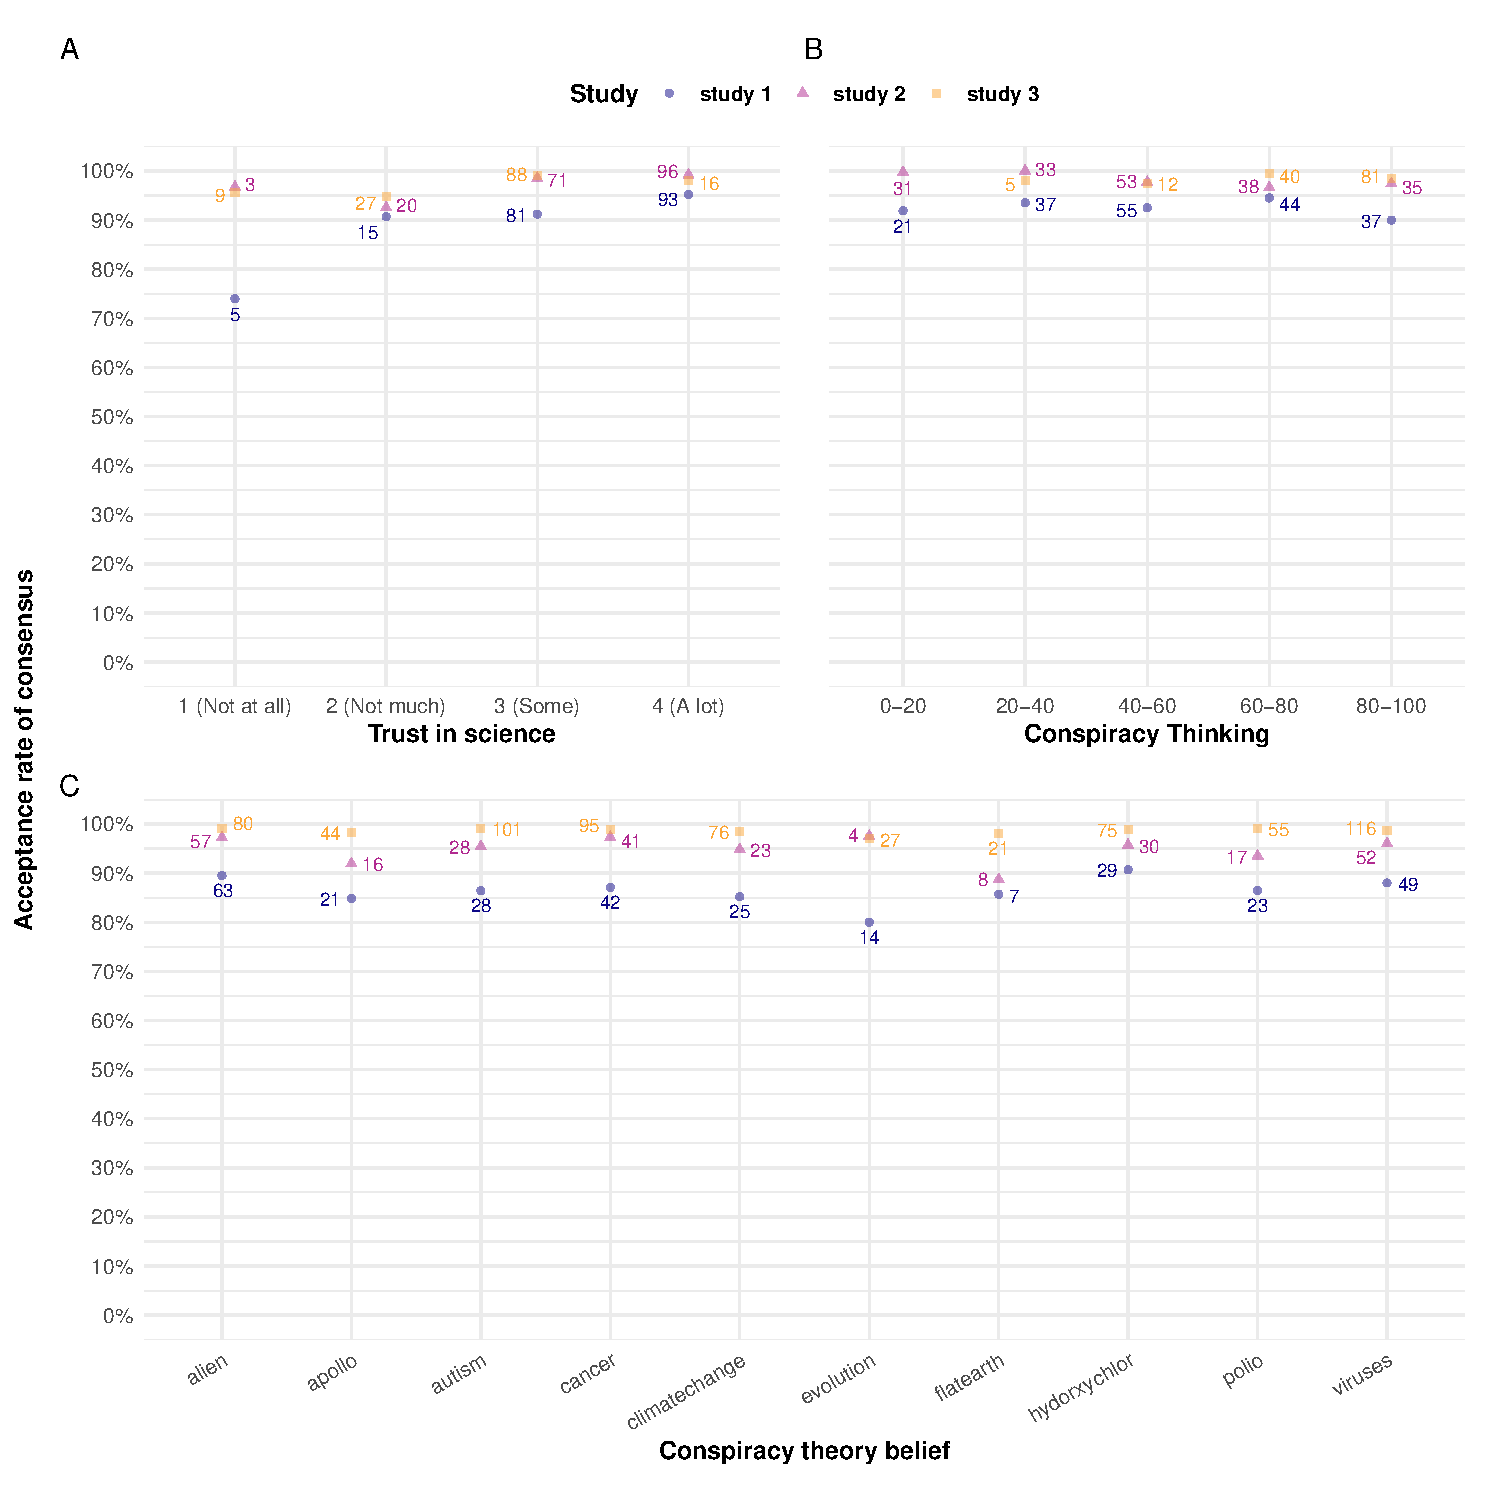
\includegraphics{output/figures/summary-plot.pdf}
\caption{\label{fig:summary-plot}Points represent the average share of acceptance and numbers the absolute count of participants as a function of: \textbf{A} the level of trust in science (``In general, would you say that you trust science a lot, some, not much, or not at all? {[}1 = Not at all, 2 = Not much, 3 = Some, 4 = A lot{]}''); \textbf{B} the average conspiracy thinking (CMQ, five items on a scale from 0 to 100); \textbf{C} the belief in specific conspiracy theories (i.e.~participants who answered 9, ``completely true'', for a given theory, see Table \ref{tab:conspiracy} for the list of the theories).}
\end{figure}

The main outcome of interest is acceptance of the scientifically consensual facts presented. Overall, acceptance was very high (aggregating across all studies: 95.1 \%; Studies 1: 93 \%; 2: 98 \%; 3: 98 \%; 4: 91 \%). Note that this includes both participants who had previously correctly answered the knowledge question, and participants who changed their mind when presented with the scientific consensus. In Studies 3 and 4, we gave participants a second chance in case they had initially rejected the consensus, which slightly increased acceptance rates in those studies (initial acceptance in Studies 3: 96 \%; 4: 86 \%).

As shown in Figure \ref{fig:summary-plot}, these very high rates of acceptance hold for: participants who do not trust science at all (4.2 \% of participants, acceptance rate of 87.3 \%), participants who rank in the top two deciles of the conspiracy thinking scale (34.3 \% of participants, acceptance rate of 93.2 \%), participants who consider as ``completely true'' (the maximum of the 9-point scale) conspiracy theories stating that the earth is flat (3.7 \% of participants, acceptance rate of 87.2 \%), or that climate change due to fossil emissions is a hoax (11.4 \% of participants, acceptance rate of 91.7 \%).

Participants in the lowest decile of acceptance still had an average acceptance rate of 67.4 \%. Even the three participants who considered as ``completely true'' that the earth is flat and who said they do ``not trust science at all'' had an average acceptance rate of 86.7 \%.

These high acceptance rates do not merely reflect science knowledge: participants only correctly answered 65.8 \% of the questions (Studies 1: 74 \%; 2: 79 \%; 3: 75 \%; 4: 36 \%) before they were provided with the scientifically consensual answer. Even the lowest decile in science knowledge, which on average answered correctly only on 20 \% of the questions, had an average acceptance rate of 91.7 \%.

Did participants who had initially provided a wrong answer change their minds towards the scientific consensus? Yes. In most cases (Studies 1: 76.3 \%; 2: 92.9 \%; 3: 95.5 \%; 4: 89.5 \%), participants readily accepted the scientific consensus after having initially given the wrong answer to a question.

How do knowledge and acceptance relate to declared general trust in science and conspiracy belief (two strongly correlated variables, pooled r = -0.64, p \textless{} .001)?

Regarding H1, we find a consistent association between trust in science and acceptance of the scientific consensus (Studies 1: r = 0.27, p \textless{} .001; 2: r = 0.30, p \textless{} .001; 3: r = 0.20, p = 0.019; 4: r = 0.16, p = 0.029), but a less consistent relation between trust in science and science knowledge (Studies 1: r = 0.29, p \textless{} .001; 2: r = 0.28, p \textless{} .001; 3: r = 0.14, p = 0.100; 4: r = 0.10, p = 0.144).

Regarding H2, the results are mixed for the relation of conspiracy beliefs (measured as the average acceptance of all the conspiracy beliefs) with both acceptance of the scientific consensus (Studies 1: r = -0.33, p \textless{} .001; 2: r = -0.37, p \textless{} .001; 3: r = -0.02, p = 0.788; 4: r = -0.05, p = 0.498) and science knowledge (Studies 1: r = -0.38, p \textless{} .001; 2: r = -0.40, p \textless{} .001; 3: r = -0.16, p = 0.055; 4: r = -0.02, p = 0.742).

n an exploratory analysis, we find that

While actual acceptance of scientific knowledge is only weakly correlated with trust in science,

Why did participants reject the scientific consensus? We collected a total of 364 answers (Studies 2: 35; 3: 74; 4: 255) from 167 (Studies 2: 25; 3: 47; 4: 95) participants to the open-ended questions on why they had rejected the scientific consensus on a particular question. Based on the answers, we created five categories (Table \ref{tab:justifications}). All individual answers can be accessed in cleaned data sheets via the OSF project page.

\begin{table}[tbp]

\begin{center}
\begin{threeparttable}

\caption{\label{tab:justifications}Justifications for rejecting the scientific consensus by category, Studies 2, 3 and 4 combined.}

\begin{tabular}{llll}
\toprule
Category & \multicolumn{1}{c}{N (instances)} & \multicolumn{1}{c}{Share (instances)} & \multicolumn{1}{c}{N (participans)*}\\
\midrule
Not convinced & 158 & 43.4\% & 70\\
No justification & 103 & 28.3\% & 51\\
Personal convictions & 43 & 11.8\% & 31\\
Mistake & 42 & 11.5\% & 34\\
Religious Beliefs & 18 & 4.9\% & 13\\
\bottomrule
\addlinespace
\end{tabular}

\begin{tablenotes}[para]
\normalsize{\textit{Note.} *Participans with at least one answer in that category}
\end{tablenotes}

\end{threeparttable}
\end{center}

\end{table}

Why did participants say they accept the scientific consensus? In Studies 3 and 4--the vaccine hesitant samples--we had asked participants about cases in which they agreed with the scientific consensus. A total of 320 (Studies 3: 122; 4: 198) participants answered this question. There were more participants saying they accepted the scientific consensus because they independently verified the fact (Studies 3: 47.5\%; 4: 47\% ), than participants saying it was because they trust scientists (Studies 3: 41.8\%; 4: 36.4\%)\footnote{10.7\% in Study 3 and 16.7\% in Study 4 answered with ``other'' and gave an open-ended explanation.}. Answers to a question about how they had done so can be found in the ESM, sections \ref{exp3} and \ref{exp4}.

In an exploratory analysis, we ran linear regressions to test whether there are differences between participants who said they had trusted science and those who said they had verified the information independently. Participants who said they accepted the consensus because of trust in scientists reported trusting science more (Studies 3: mean = 3; \(\hat{\beta}_{\text{Trust}}\) = 0.19, p = 0.330 on a scale from 1 to 4; 4: mean = 2.92; \(\hat{\beta}_{\text{Trust}}\) = 0.46, p \textless{} .001) than those who said they verified independently (Studies 3 mean = 2.81; 4: mean = 2.45). We did not find a difference regarding acceptance (Studies 3: \(\hat{\beta}_{\text{Acceptance}}\) = 0.01, p = 0.523 on a scale from 0 to 1; 4: \(\hat{\beta}_{\text{Acceptance}}\) = 0.04, p = 0.116) or regarding beliefs in conspiracy theories (Studies 3: \(\hat{\beta}_{\text{BCTI}}\) = -0.16, p = 0.694 on a scale from 1 to 9; 4: \(\hat{\beta}_{\text{BCTI}}\) = -0.21, p = 0.322). We also did not find a difference in time spent on the survey in Study 3 (\(\hat{\beta}_{\text{Time}}\) = -0.02, p = 0.985; median = 7.64 mins), but in Study 4, people who said they had accepted the consensus because they they trust scientists tended to spend on average two minutes less on the survey (\(\hat{\beta}_{\text{Time}}\) = -2.16, p = 0.018; median = 9.38 mins).\footnote{For these analyses, we excluded outliers who took over 30 mins for the survey, which was estimated to take around 10 mins, and for which the median time was seven minutes. As a result, we excluded one participant in Study 3 and four in Study 4. Significance levels are not affected by these exclusions.} In Study 4, in which we used facts that participants were unlikely to have encountered before, we tracked whether people clicked on the source links provided--a behavior that you would expect from people who report verifying facts independently. On average, participants clicked only on 1.36 links (out of 20 possible clicks) and there was no difference between the two groups (\(\hat{\beta}_{\text{Clicks}}\) = -1.09, p = 0.062).

More detailed results addressing all our pre-registered research questions can be found in the ESM, sections \ref{exp1} to \ref{exp4}.

\section{Discussion}\label{discussion}

In four studies, we asked US participants whether they accepted scientifically consensual answers on basic science questions. We found quasi-universal acceptance of basic science, with an overall rate of acceptance of 95.1 \%, which remained very high for participants who declared not trusting science at all (87.3 \% of acceptance), or who endorsed theories blatantly violating scientific knowledge, such as flat earth (87.2 \% of acceptance).

This disconnect between declared general trust in science and average trust in (basic) scientific findings goes against predictions from the knowledge--attitudes model of trust in science (see, e.g., Bauer, Allum, \& Miller, 2007), which posits that knowledge of scientific results is the main cause of trust in science. In line with past research (Allum et al., 2008), we find that both knowledge and acceptance of science are only weakly correlated with general trust in science. This supports contemporary definitions of science literacy, which suggest that for science literacy to be a meaningful concept for science attitudes, it needs to go beyond measuring knowledge of isolated science facts (National Academies of Sciences, Engineering, and Medicine, 2016).

Instead, our findings align with a motivated reasoning account of trust in science (Lewandowsky \& Oberauer, 2016), in which ``people tend to reject findings that threaten their core beliefs or worldview'' (p.~217). A number of participants in our studies endorsed specific conspiracy theories questioning basic tenets of science (on evolution, the shape of the earth, etc.), while still accepting the vast majority of basic scientific facts presented to them. This suggests that these participants had reasons to reject only specific scientific knowledge, and that this rejection prompted them to express a lower trust in science when asked general questions on the topic. Consistent with this explanation, we found a strong association between belief in the anti-science conspiracy theories and general trust in science.

Some of the present results also speak to the alienation model (Gauchat, 2011), and more specifically to the need for epistemic autonomy (Fricker, 2006). Declaring not trusting science, or endorsing conspiracy theories (Harris, 2023) might reflect a desire to maintain epistemic autonomy and not appear to `blindly' accept epistemic authority. Such a need to appear epistemically autonomous would be reconciled with the acceptance of basic science facts if it stems from independent evaluation instead of trust. The majority of participants in Studies 3 and 4, two samples of vaccine skeptical participants who scored high across a range of different conspiracy beliefs (see ESM), claimed that this was their case, however implausible that might be: it's not clear how participants could independently verify, say, the ratio of glial cells to neurons. These participants did also not engage any more in simple forms of verification, i.e.~clicking on sources provided in the answers. This aligns with other results on conspiracy thinking: Several recent studies have shown that, although they claim not to be, conspiracy theorists are in fact just as susceptible to social influence as others (Altay, Nera, Ejaz, Schöpfer, \& Tomas, 2023; Pummerer, Fock, Winter, \& Sassenberg, 2024).

In applied terms, the present results have implications for science communication. Across various domains of science knowledge such as climate change (Većkalov et al., 2024) or vaccination (Salmon, Dudley, Glanz, \& Omer, 2015), researchers have observed a consensus gap: a gap between the scientific consensus and public opinion. For example, some of the most worrying consensus gaps relate to climate change, as substantial segments of the population disagree with scientists on what is happening and what to do about it (e.g., Egan \& Mullin, 2017). Yet, we found that for much of basic, non-contentious science, such consensus gaps are absent: The vast majority of our participants--including two vaccine-skeptic attitudes samples (Studies 3 and 4)--did not appear to have general grounds for distrusting science, which should have led them to reject most or all of the science knowledge presented to them. Since even people who distrust science or reject contentious science facts appear to accept most of basic science, stressing the basic science components of publicly controversial fields, from GMOs to climate change, might help reduce the consensus gaps observed in these domains (on climate change, see, e.g. Ranney \& Clark, 2016).

The present studies have a number of limitations, in particular the lack of representative samples, and the focus on a single country. While our results lend support to motivated reasoning accounts of trust in science, they leave several important questions unaddressed, in particular: Why do people reject specific science beliefs but not others? Suggestions have already been made for a number of issues such as vaccination (Miton \& Mercier, 2015), GMOs (Blancke, Van Breusegem, De Jaeger, Braeckman, \& Van Montagu, 2015), or nuclear energy (Hacquin, Altay, Aarøe, \& Mercier, 2021). However, research is still needed to better understand what motivates these rejections (see e.g., Hornsey, 2020). Moreover, rejection of scientific facts can manifest in various ways, for example calling into question the integrity of scientists (Mede, 2023; Mede, Schäfer, Metag, \& Klinger, 2022), or denying the very possibility of scientifically investigating certain issues (Munro, 2010). The classification of justifications we present here does not address these processes in detail. Finally, by design, most of the basic science knowledge presented in this study didn't directly relate to anything controversial for most people. Future studies could look at basic science that does relate to science topics which are the object of public and policy-relevant debates (e.g.~GM food, climate science, vaccines), or scientific findings for which there is a more obvious potential conflict of interest (e.g.~non-publicly funded medical research).

\FloatBarrier

\section{References}\label{references}

\phantomsection\label{refs}
\begin{CSLReferences}{1}{0}
\bibitem[\citeproctext]{ref-alganTrustScientistsTimes2021}
Algan, Y., Cohen, D., Davoine, E., Foucault, M., \& Stantcheva, S. (2021). Trust in scientists in times of pandemic: Panel evidence from 12 countries. \emph{Proceedings of the National Academy of Sciences}, \emph{118}(40), e2108576118. \url{https://doi.org/10.1073/pnas.2108576118}

\bibitem[\citeproctext]{ref-allumScienceKnowledgeAttitudes2008}
Allum, N., Sturgis, P., Tabourazi, D., \& Brunton-Smith, I. (2008). Science knowledge and attitudes across cultures: a meta-analysis. \emph{Public Understanding of Science}, \emph{17}(1), 35--54. \url{https://doi.org/10.1177/0963662506070159}

\bibitem[\citeproctext]{ref-altayConspiracyBelieversClaim2023}
Altay, S., Nera, K., Ejaz, W., Schöpfer, C., \& Tomas, F. (2023). Conspiracy believers claim to be free thinkers but (Under)Use advice like everyone else. \emph{British Journal of Social Psychology}, \emph{62}(4), 1782--1797. \url{https://doi.org/10.1111/bjso.12655}

\bibitem[\citeproctext]{ref-altenmullerExplainingPolarizedTrust2024}
Altenmüller, M. S., Wingen, T., \& Schulte, A. (2024). Explaining Polarized Trust in Scientists: A Political Stereotype-Approach. \emph{Science Communication}, \emph{46}(1), 92--115. \url{https://doi.org/10.1177/10755470231221770}

\bibitem[\citeproctext]{ref-bauerWhatCanWe2007}
Bauer, M. W., Allum, N., \& Miller, S. (2007). What can we learn from 25 years of PUS survey research? Liberating and expanding the agenda. \emph{Public Understanding of Science}, \emph{16}(1), 79--95. \url{https://doi.org/10.1177/0963662506071287}

\bibitem[\citeproctext]{ref-besleyReassessingVariablesUsed2021}
Besley, J. C., Lee, N. M., \& Pressgrove, G. (2021). Reassessing the Variables Used to Measure Public Perceptions of Scientists. \emph{Science Communication}, \emph{43}(1), 3--32. \url{https://doi.org/10.1177/1075547020949547}

\bibitem[\citeproctext]{ref-blanckeFatalAttractionIntuitive2015}
Blancke, S., Van Breusegem, F., De Jaeger, G., Braeckman, J., \& Van Montagu, M. (2015). Fatal attraction: the intuitive appeal of GMO opposition. \emph{Trends in Plant Science}, \emph{20}(7), 414--418. \url{https://doi.org/10.1016/j.tplants.2015.03.011}

\bibitem[\citeproctext]{ref-brianAmericansTrustScientists2023}
Brian, K., \& Tyson, A. (2023). \emph{Americans{'} trust in scientists, positive views of science continue to decline}. Retrieved from \url{https://www.pewresearch.org/science/2023/11/14/americans-trust-in-scientists-positive-views-of-science-continue-to-decline/}

\bibitem[\citeproctext]{ref-bruderMeasuringIndividualDifferences2013}
Bruder, M., Haffke, P., Neave, N., Nouripanah, N., \& Imhoff, R. (2013). Measuring individual differences in generic beliefs in conspiracy theories across cultures: Conspiracy mentality questionnaire. \emph{Frontiers in Psychology}, \emph{4}. Retrieved from \url{https://www.frontiersin.org/articles/10.3389/fpsyg.2013.00225}

\bibitem[\citeproctext]{ref-colognaTrustScientistsTheir2024}
Cologna, V., Mede, N. G., Berger, S., Besley, J., Brick, C., Joubert, M., \ldots{} Linden, D. S. van der. (2024). \emph{Trust in scientists and their role in society across 67 countries}. \url{https://doi.org/10.31219/osf.io/6ay7s}

\bibitem[\citeproctext]{ref-colognaRoleTrustClimate2020}
Cologna, V., \& Siegrist, M. (2020). The role of trust for climate change mitigation and adaptation behaviour: A meta-analysis. \emph{Journal of Environmental Psychology}, \emph{69}, 101428. \url{https://doi.org/10.1016/j.jenvp.2020.101428}

\bibitem[\citeproctext]{ref-douglasUnderstandingConspiracyTheories2019}
Douglas, K. M., Uscinski, J. E., Sutton, R. M., Cichocka, A., Nefes, T., Ang, C. S., \& Deravi, F. (2019). Understanding Conspiracy Theories. \emph{Political Psychology}, \emph{40}(S1), 3--35. \url{https://doi.org/10.1111/pops.12568}

\bibitem[\citeproctext]{ref-durantPublicUnderstandingScience1989}
Durant, J. R., Evans, G. A., \& Thomas, G. P. (1989). The public understanding of science. \emph{Nature}, \emph{340}(6228), 11--14. \url{https://doi.org/10.1038/340011a0}

\bibitem[\citeproctext]{ref-eganClimateChangeUS2017}
Egan, P. J., \& Mullin, M. (2017). Climate change: US public opinion. \emph{Annual Review of Political Science}, \emph{20}, 209--227.

\bibitem[\citeproctext]{ref-fernbachExtremeOpponentsGenetically2019}
Fernbach, P. M., Light, N., Scott, S. E., Inbar, Y., \& Rozin, P. (2019). Extreme opponents of genetically modified foods know the least but think they know the most. \emph{Nature Human Behaviour}, \emph{3}(3), 251--256. \url{https://doi.org/10.1038/s41562-018-0520-3}

\bibitem[\citeproctext]{ref-frickerTestimonyEpistemicAutonomy2006}
Fricker, E. (2006). \emph{Testimony and Epistemic Autonomy} (J. Lackey \& E. Sosa, Eds.). Oxford University PressOxford. \url{https://doi.org/10.1093/acprof:oso/9780199276011.003.0011}

\bibitem[\citeproctext]{ref-funkKeyFindingsPublic2019}
Funk, C., Johnson, C., \& Hefferon, M. (2019). \emph{5 key findings about public trust in scientists in the u.s.} Retrieved from \url{https://www.pewresearch.org/fact-tank/2019/08/05/5-key-findings-about-public-trust-in-scientists-in-the-u-s/}

\bibitem[\citeproctext]{ref-funkPublicConfidenceScientists2020}
Funk, C., \& Kennedy, B. (2020). \emph{Public confidence in scientists has remained stable for decades}.

\bibitem[\citeproctext]{ref-gauchatCulturalAuthorityScience2011}
Gauchat, G. (2011). The cultural authority of science: Public trust and acceptance of organized science. \emph{Public Understanding of Science}, \emph{20}(6), 751--770. \url{https://doi.org/10.1177/0963662510365246}

\bibitem[\citeproctext]{ref-gauchatPoliticizationSciencePublic2012}
Gauchat, G. (2012). Politicization of Science in the Public Sphere: A Study of Public Trust in the United States, 1974 to 2010. \emph{American Sociological Review}, \emph{77}(2), 167--187. \url{https://doi.org/10.1177/0003122412438225}

\bibitem[\citeproctext]{ref-gauchatCulturalCognitiveMappingScientific2018}
Gauchat, G., \& Andrews, K. T. (2018). The Cultural-Cognitive Mapping of Scientific Professions. \emph{American Sociological Review}, \emph{83}(3), 567--595. \url{https://doi.org/10.1177/0003122418773353}

\bibitem[\citeproctext]{ref-gligoricHowSocialEvaluations2024}
Gligorić, V., Kleef, G. A. van, \& Rutjens, B. T. (2024). How social evaluations shape trust in 45 types of scientists. \emph{PLOS ONE}, \emph{19}(4), e0299621. \url{https://doi.org/10.1371/journal.pone.0299621}

\bibitem[\citeproctext]{ref-hacquinDisgustSensitivityPublic2021}
Hacquin, A.-S., Altay, S., Aarøe, L., \& Mercier, H. (2021). Disgust sensitivity and public opinion on nuclear energy. \emph{Journal of Environmental Psychology}, 101749.

\bibitem[\citeproctext]{ref-harrisConspiracyTheoriesPopulism2023}
Harris, K. R. (2023). Conspiracy Theories, Populism, and Epistemic Autonomy. \emph{Journal of the American Philosophical Association}, \emph{9}(1), 21--36. \url{https://doi.org/10.1017/apa.2021.44}

\bibitem[\citeproctext]{ref-hendriksMeasuringLaypeoplesTrust2015}
Hendriks, F., Kienhues, D., \& Bromme, R. (2015). Measuring Laypeople{'}s Trust in Experts in a Digital Age: The Muenster Epistemic Trustworthiness Inventory (METI). \emph{PLOS ONE}, \emph{10}(10), e0139309. \url{https://doi.org/10.1371/journal.pone.0139309}

\bibitem[\citeproctext]{ref-hornseyWhyFactsAre2020}
Hornsey, M. J. (2020). Why Facts Are Not Enough: Understanding and Managing the Motivated Rejection of Science. \emph{Current Directions in Psychological Science}, \emph{29}(6), 583--591. \url{https://doi.org/10.1177/0963721420969364}

\bibitem[\citeproctext]{ref-hornseyAttitudeRootsJiu2017}
Hornsey, M. J., \& Fielding, K. S. (2017). Attitude roots and Jiu Jitsu persuasion: Understanding and overcoming the motivated rejection of science. \emph{American Psychologist}, \emph{72}(5), 459--473. \url{https://doi.org/10.1037/a0040437}

\bibitem[\citeproctext]{ref-hornseyRelationshipsConspiratorialBeliefs2018}
Hornsey, M. J., Harris, E. A., \& Fielding, K. S. (2018a). Relationships among conspiratorial beliefs, conservatism and climate scepticism across nations. \emph{Nature Climate Change}, \emph{8}(7), 614--620. \url{https://doi.org/10.1038/s41558-018-0157-2}

\bibitem[\citeproctext]{ref-hornseyPsychologicalRootsAntivaccination2018}
Hornsey, M. J., Harris, E. A., \& Fielding, K. S. (2018b). The psychological roots of anti-vaccination attitudes: A 24-nation investigation. \emph{Health Psychology}, \emph{37}(4), 307--315. \url{https://doi.org/10.1037/hea0000586}

\bibitem[\citeproctext]{ref-intemannScienceCommunicationPublic2023}
Intemann, K. (2023). Science communication and public trust in science. \emph{Interdisciplinary Science Reviews}, \emph{48}(2), 350--365. \url{https://doi.org/10.1080/03080188.2022.2152244}

\bibitem[\citeproctext]{ref-krauseTrendsAmericansTrust2019a}
Krause, N. M., Brossard, D., Scheufele, D. A., Xenos, M. A., \& Franke, K. (2019). Trends{\textemdash}americans{'} trust in science and scientists. \emph{Public Opinion Quarterly}, \emph{83}(4), 817--836. \url{https://doi.org/10.1093/poq/nfz041}

\bibitem[\citeproctext]{ref-lantianMeasuringBeliefConspiracy2016}
Lantian, A., Muller, D., Nurra, C., \& Douglas, K. M. (2016). Measuring Belief in Conspiracy Theories: Validation of a French and English Single-Item Scale. \emph{International Review of Social Psychology}, \emph{29}(1), 1. \url{https://doi.org/10.5334/irsp.8}

\bibitem[\citeproctext]{ref-lewandowskyRoleConspiracistIdeation2013}
Lewandowsky, S., Gignac, G. E., \& Oberauer, K. (2013). The Role of Conspiracist Ideation and Worldviews in Predicting Rejection of Science. \emph{PLOS ONE}, \emph{8}(10), e75637. \url{https://doi.org/10.1371/journal.pone.0075637}

\bibitem[\citeproctext]{ref-lewandowskyMotivatedRejectionScience2016}
Lewandowsky, S., \& Oberauer, K. (2016). Motivated Rejection of Science. \emph{Current Directions in Psychological Science}, \emph{25}(4), 217--222. \url{https://doi.org/10.1177/0963721416654436}

\bibitem[\citeproctext]{ref-liPolarizationPublicTrust2022}
Li, N., \& Qian, Y. (2022). Polarization of public trust in scientists between 1978 and 2018: Insights from a cross-decade comparison using interpretable machine learning. \emph{Politics and the Life Sciences}, \emph{41}(1), 45--54. \url{https://doi.org/10.1017/pls.2021.18}

\bibitem[\citeproctext]{ref-lindholtPublicAcceptanceCOVID192021}
Lindholt, M. F., Jørgensen, F., Bor, A., \& Petersen, M. B. (2021). Public acceptance of COVID-19 vaccines: cross-national evidence on levels and individual-level predictors using observational data. \emph{BMJ Open}, \emph{11}(6), e048172. \url{https://doi.org/10.1136/bmjopen-2020-048172}

\bibitem[\citeproctext]{ref-mayerIntegrativeModelOrganizational1995a}
Mayer, R. C., Davis, J. H., \& Schoorman, F. D. (1995). An Integrative Model of Organizational Trust. \emph{The Academy of Management Review}, \emph{20}(3), 709. \url{https://doi.org/10.2307/258792}

\bibitem[\citeproctext]{ref-medeSciencerelatedPopulismConceptualization2023a}
Mede, N. G. (2023). Science-related populism: Conceptualization, empirical investigation, and implications for science communication (Dissertation Summary). \emph{Studies in Communication Sciences}, \emph{23}(3). \url{https://doi.org/10.24434/j.scoms.2023.03.4403}

\bibitem[\citeproctext]{ref-medeSciencerelatedPopulismConceptualizing2020}
Mede, N. G., \& Schäfer, M. S. (2020). Science-related populism: Conceptualizing populist demands toward science. \emph{Public Understanding of Science}, \emph{29}(5), 473--491. \url{https://doi.org/10.1177/0963662520924259}

\bibitem[\citeproctext]{ref-medeWhoSupportsSciencerelated2022}
Mede, N. G., Schäfer, M. S., Metag, J., \& Klinger, K. (2022). Who supports science-related populism? A nationally representative survey on the prevalence and explanatory factors of populist attitudes toward science in Switzerland. \emph{PLOS ONE}, \emph{17}(8), e0271204. \url{https://doi.org/10.1371/journal.pone.0271204}

\bibitem[\citeproctext]{ref-millerMeasurementCivicScientific1998a}
Miller, J. D. (1998). The measurement of civic scientific literacy. \emph{Public Understanding of Science}, \emph{7}(3), 203--223. \url{https://doi.org/10.1088/0963-6625/7/3/001}

\bibitem[\citeproctext]{ref-mitonCognitiveObstaclesProVaccination2015}
Miton, H., \& Mercier, H. (2015). Cognitive Obstacles to Pro-Vaccination Beliefs. \emph{Trends in Cognitive Sciences}, \emph{19}(11), 633--636. \url{https://doi.org/10.1016/j.tics.2015.08.007}

\bibitem[\citeproctext]{ref-munroScientificImpotenceExcuse2010}
Munro, G. D. (2010). The scientific impotence excuse: Discounting belief-threatening scientific abstracts. \emph{Journal of Applied Social Psychology}, \emph{40}(3), 579--600. \url{https://doi.org/10.1111/j.1559-1816.2010.00588.x}

\bibitem[\citeproctext]{ref-nadelsonTrustScienceScientists2015}
Nadelson, L. S., \& Hardy, K. K. (2015). Trust in science and scientists and the acceptance of evolution. \emph{Evolution: Education and Outreach}, \emph{8}(1), 9. \url{https://doi.org/10.1186/s12052-015-0037-4}

\bibitem[\citeproctext]{ref-nationalacademiesofsciencesengineeringandmedicineScienceLiteracyConcepts2016}
National Academies of Sciences, Engineering, and Medicine. (2016). \emph{Science Literacy: Concepts, Contexts, and Consequences} (C. E. Snow \& K. A. Dibner, Eds.). Washington, D.C.: National Academies Press. \url{https://doi.org/10.17226/23595}

\bibitem[\citeproctext]{ref-pennycookOverconfidentlyConspiratorialConspiracy2022}
Pennycook, G., Binnendyk, J., \& Rand, D. (2022). \emph{Overconfidently conspiratorial: Conspiracy believers are dispositionally overconfident and massively overestimate how much others agree with them}. \url{https://doi.org/10.31234/osf.io/d5fz2}

\bibitem[\citeproctext]{ref-pummererConspiracyBeliefsMajority2024}
Pummerer, L., Fock, L., Winter, K., \& Sassenberg, K. (2024). Conspiracy beliefs and majority influence. \emph{The Journal of Social Psychology}, 1--16. \url{https://doi.org/10.1080/00224545.2024.2397491}

\bibitem[\citeproctext]{ref-ranneyClimateChangeConceptual2016}
Ranney, M. A., \& Clark, D. (2016). Climate Change Conceptual Change: Scientific Information Can Transform Attitudes. \emph{Topics in Cognitive Science}, \emph{8}(1), 49--75. \url{https://doi.org/10.1111/tops.12187}

\bibitem[\citeproctext]{ref-rousseauIntroductionSpecialTopic1998}
Rousseau, D. M., Sitkin, S. B., Burt, R. S., \& Camerer, C. (1998). Introduction to Special Topic Forum: Not so Different after All: A Cross-Discipline View of Trust. \emph{The Academy of Management Review}, \emph{23}(3), 393--404. Retrieved from \url{http://www.jstor.org/stable/259285}

\bibitem[\citeproctext]{ref-rutjensConspiracyBeliefsScience2022}
Rutjens, B. T., \& Većkalov, B. (2022). Conspiracy beliefs and science rejection. \emph{Current Opinion in Psychology}, \emph{46}, 101392. \url{https://doi.org/10.1016/j.copsyc.2022.101392}

\bibitem[\citeproctext]{ref-salmonVaccineHesitancyCauses2015}
Salmon, D. A., Dudley, M. Z., Glanz, J. M., \& Omer, S. B. (2015). Vaccine hesitancy: Causes, consequences, and a call to action. \emph{Vaccine}, \emph{33}, D66--D71.

\bibitem[\citeproctext]{ref-stockemerUnderstandingClimateChange2024}
Stockemer, D., \& Bordeleau, J.-N. (2024). Understanding climate change conspiracy beliefs: A comparative outlook. \emph{Harvard Kennedy School Misinformation Review}, \emph{5}(6). \url{https://doi.org/10.37016/mr-2020-162}

\bibitem[\citeproctext]{ref-sturgisTrustScienceSocial2021}
Sturgis, P., Brunton-Smith, I., \& Jackson, J. (2021). Trust in science, social consensus and vaccine confidence. \emph{Nature Human Behaviour}, \emph{5}(11), 1528--1534. \url{https://doi.org/10.1038/s41562-021-01115-7}

\bibitem[\citeproctext]{ref-uscinskiHaveBeliefsConspiracy2022}
Uscinski, J., Enders, A., Klofstad, C., Seelig, M., Drochon, H., Premaratne, K., \& Murthi, M. (2022). Have beliefs in conspiracy theories increased over time? \emph{PLoS ONE}, \emph{17}(7), e0270429. \url{https://doi.org/10.1371/journal.pone.0270429}

\bibitem[\citeproctext]{ref-vanstekelenburgScientificConsensusCommunicationContested2022}
Van Stekelenburg, A., Schaap, G., Veling, H., Van 'T Riet, J., \& Buijzen, M. (2022). Scientific-Consensus Communication About Contested Science: A Preregistered Meta-Analysis. \emph{Psychological Science}, \emph{33}(12), 1989--2008. \url{https://doi.org/10.1177/09567976221083219}

\bibitem[\citeproctext]{ref-veckalov27countryTestCommunicating2024}
Većkalov, B., Geiger, S. J., Bartoš, F., White, M. P., Rutjens, B. T., Harreveld, F. van, \ldots{} Linden, S. van der. (2024). A 27-country test of communicating the scientific consensus on climate change. \emph{Nature Human Behaviour}, 1--14. \url{https://doi.org/10.1038/s41562-024-01928-2}

\bibitem[\citeproctext]{ref-vranicDidMyOwn2022}
Vranic, A., Hromatko, I., \& Tonković, M. (2022). {``}I did my own research{''}: Overconfidence, (dis)trust in science, and endorsement of conspiracy theories. \emph{Frontiers in Psychology}, \emph{13}. \url{https://doi.org/10.3389/fpsyg.2022.931865}

\bibitem[\citeproctext]{ref-wellcomeglobalmonitorWellcomeGlobalMonitor2018}
Wellcome Global Monitor. (2018). \emph{Wellcome Global Monitor 2018}. Retrieved from \url{https://wellcome.org/reports/wellcome-global-monitor/2018}

\bibitem[\citeproctext]{ref-wellcomeglobalmonitorWellcomeGlobalMonitor2020}
Wellcome Global Monitor. (2020). \emph{Wellcome Global Monitor 2020: Covid-19}. Retrieved from \url{https://wellcome.org/reports/wellcome-global-monitor-covid-19/2020}

\bibitem[\citeproctext]{ref-wellcomeglobalmonitorPublicTrustScientists2021}
Wellcome Global Monitor. (2021). \emph{Public trust in scientists rose during the Covid-19 pandemic \textbar{} News}. Retrieved from \url{https://wellcome.org/news/public-trust-scientists-rose-during-covid-19-pandemic}

\bibitem[\citeproctext]{ref-wilholtEpistemicTrustScience2013}
Wilholt, T. (2013). Epistemic trust in science. \emph{The British Journal for the Philosophy of Science}, \emph{64}(2), 233--253. \url{https://doi.org/10.1093/bjps/axs007}

\bibitem[\citeproctext]{ref-wintterlinPredictingPublicTrust2022}
Wintterlin, F., Hendriks, F., Mede, N. G., Bromme, R., Metag, J., \& Schäfer, M. S. (2022). Predicting public trust in science: The role of basic orientations toward science, perceived trustworthiness of scientists, and experiences with science. \emph{Frontiers in Communication}, \emph{6}. \url{https://doi.org/10.3389/fcomm.2021.822757}

\end{CSLReferences}

\newpage

\newpage

\appendix


\section{Acceptance conditional on knowledge}\label{acceptance-knowledge}

Did participants who gave a wrong answer change their minds towards the scientific consensus? In most cases (Studies 1: 76.3 \%; 2: 92.9 \%; 3: 95.5 \%; 4: 89.5 \%), participants readily accepted the scientific consensus after having initially given the wrong answer to a question. In very few cases, participants changed their mind away from the scientific consensus. These participants initially gave the correct response, but rejected the scientific consensus right after, thereby contradicting their own initial response (Studies 1: 1.6 \%; 2: 0.5 \%; 3: 0.7 \%; 4: 5.7 \%). Figure \ref{fig:acceptance-knowledge} shows acceptance rates conditional on whether the initial answer to the questions was correct or not.



\begin{figure}
\centering
\includegraphics{output/figures/acceptance-knowledge.pdf}
\caption{\label{fig:acceptance-knowledge}Acceptance/Rejection rate of scientific consensus, based on whether the initial response to the knowledge question was false or true.}
\end{figure}

\clearpage

\section{Conspiracy Thinking}\label{conspiracy-thinking}

Figure \ref{fig:conspiracy-thinking-overview} shows the distributions of conspiracy thinking across the four studies.



\begin{figure}
\centering
\includegraphics{output/figures/conspiracy-thinking-overview.pdf}
\caption{\label{fig:conspiracy-thinking-overview}Distributions of conspiracy thinking.}
\end{figure}

\clearpage

\section{Trust in science}\label{trust}

Figure \ref{fig:trust-overview} shows the distributions of our main trust in science measure across the four studies.



\begin{figure}
\centering
\includegraphics{output/figures/trust-overview.pdf}
\caption{\label{fig:trust-overview}Distributions of trust in science.}
\end{figure}

\clearpage

\section{Conspiracy Belief}\label{conspiracy-belief}

Figure \ref{fig:conspiracy-belief-overview} shows the average belief in each of the conspiracy theories across the four studies.



\begin{figure}
\centering
\includegraphics{output/figures/conspiracy-belief-overview.pdf}
\caption{\label{fig:conspiracy-belief-overview}Average belief in conspiracy theories.}
\end{figure}

\clearpage

\section{Science knowledge}\label{knowledge}

Figure \ref{fig:knowledge-overview} shows the distributions of basic science knowledge across the four studies.

Were participants better than chance in their answers? To obtain the expected value (EV) of someone answering at random, for each question, we calculate the probability of answering correctly (since each correct answer gives 1 point), and then sum these probabilities. In the case of Study 1, the EV is 4.666667 out of 11 (1/3 + 1/3 + 1/2 + 1/3 + 1/2 + 1/3 + 1/2 + 1/2 + 1/2 + 1/2 + 1/3) including the additional item on where trees draw most of their materials from. Without this item, the EV is, just as in Studies 2 and 3, 4.333333 out of 10 (1/3 + 1/3 + 1/2 + 1/3 + 1/2 + 1/3 + 1/2 + 1/2 + 1/2 + 1/2). In Study 4 the number of answer options was consistently three, so the EV is 3.333333.

As visualized in Figure \ref{fig:knowledge-overview}, for Studies 1, 2, and 3, the vast majority of participants obtained a higher score than the EV, strongly suggesting answers not at random. For Study 4, as expected from the very specific, non-standard questions, the knowledge score is centered around the EV, suggesting that most people were at random, and slightly right-skewed, suggesting that a few individuals were either very knowledgeable or looked up some of the answers.



\begin{figure}
\centering
\includegraphics{output/figures/knowledge-overview.pdf}
\caption{\label{fig:knowledge-overview}Distributions of science knowledge.}
\end{figure}

\clearpage

\section{Acceptance and knowledge by question}\label{by-question-variation}

Figure \ref{fig:knowledge-overview} shows the share of correct answers, and Figure \ref{fig:knowledge-overview} the acceptance rate of the scientific consensus, for each knowledge question asked in the respective study.



\begin{figure}
\centering
\includegraphics{output/figures/questions-knowledge.pdf}
\caption{\label{fig:questions-knowledge}Share of correct answers by question.}
\end{figure}



\begin{figure}
\centering
\includegraphics{output/figures/questions-acceptance.pdf}
\caption{\label{fig:questions-acceptance}Acceptance rate of consensus by question.}
\end{figure}

\clearpage

\section{Conspiracy Measures}\label{exp1}

In addition to the Belief in Conspiracy Theory Inventory (BCTI) by Pennycook et al. (2022) which report in the main study, we also assessed two other consipiracy thinking measures: The conspiracy mentality questionnaire (CMQ) by Bruder et al. (2013) and the Single Item Conspiracy Beliefs Scale (SICBS) by Lantian et al. (2016) (Table \ref{tab:overview-conspiracy-measures}).

\begingroup\fontsize{8}{10}\selectfont

\begin{longtable}[t]{>{\raggedright\arraybackslash}p{10em}>{\raggedright\arraybackslash}p{20em}>{\raggedright\arraybackslash}p{10em}}
\caption{\label{tab:overview-conspiracy-measures}Conspiracy measures}\\
\toprule
Measure & Description & Scale\\
\midrule
Belief in Conspiracy Theory Inventory (BCTI) & By Pennycook et al., 2022, presented in the main article. & 1 - 9 (1 = Completely false, 5 = Unsure, 9 = Completely true)\\
Conspiracy Mentality Questionnaire (CMQ) & By Bruder et al., 2013. Respondents are asked how much they agree with the following statements: & 0\% - 100\% (0 = certainly not, 100 = certain)\\
 & - Many important things happen in the world, which the public is never informed about. & \\
 & - Politicians usually do not tell us the true motives for their decisions. & \\
 & - Government agencies closely monitor all citizens. & \\
\addlinespace
 & - Events which seem unrelated are often the result of secret activities. & \\
 & - There are secret organizations that greatly influence political decisions. & \\
Single Item Conspiracy Beliefs Scale (SICBS) & By Lantian et al., 2016. The item is: 'I think that the official version of events given by the authorities very often hides the truth.' & 1 - 9 (1 = Completely false, 5 = Unsure, 9 = Completely true)\\
\bottomrule
\end{longtable}
\endgroup{}

\clearpage

\section{Study 1}\label{exp1}

\subsection{Participants}\label{participants-1}

We recruited 200 participants from the US via prolific. 6 participants failed our attention check, resulting in a final sample of 194 participants (98 female, 96 male; \(age_\text{mean}\): 41.71, \(age_\text{sd}\): 13.07, \(age_\text{median}\): 39). Since we did not have any prior assumptions on effect sizes, we did not do a power analysis.

\subsection{Materials}\label{materials-2}

\FloatBarrier



\begin{figure}

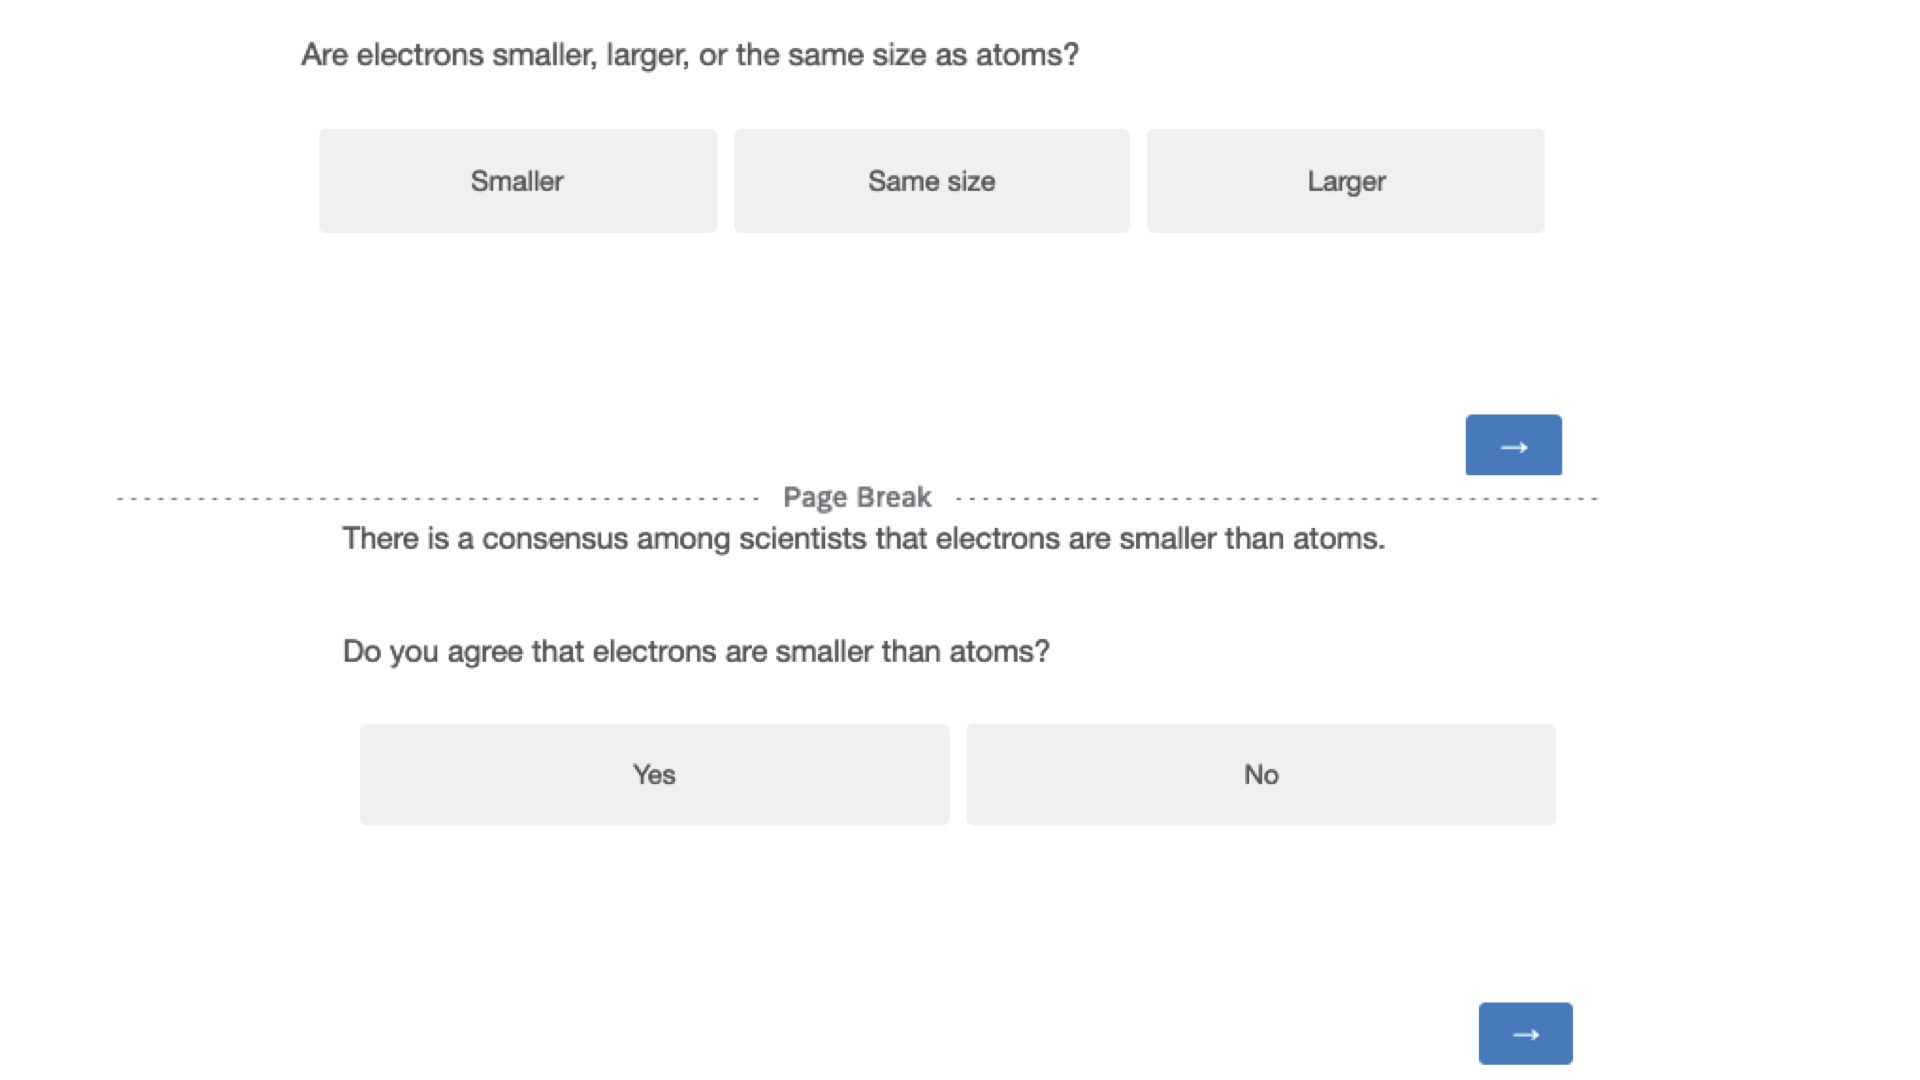
\includegraphics[width=1\linewidth]{./figures/study1_question_example} \hfill{}

\caption{Example of a science question, the scientific consensus and the corresponding acceptance question.}\label{fig:stimulus-example}
\end{figure}

\subsection{Results}\label{results-1}

Regarding RQ1 and RQ2, participants answered on average 74 \% (sd = 0.16) of the questions correctly, and accepted the scientific consensus on average for 93 \% (sd = 0.12) of the questions.

In most cases (76.3 \%), participants readily accepted the scientific consensus after having given the wrong answer to a question. In very few cases (1.6 \%), participants who gave the correct response afterwards rejected the scientific consensus, thereby contradicting their own initial response. We believe this might have been due to inattention.

For RQ3, we find a positive but small correlation between both science knowledge and trust in science (r = 0.29, p \textless{} .001), and acceptance of scientific consensus and trust in science (r = 0.27, p \textless{} .001). The more people are knowledgeable about science and the more they tend to accept the scientific consensus, the more they tend to trust science. These correlations are relatively weak, which might be partly due to ceiling effects: As illustrated in Fig. \ref{fig:exp1-plot-overview}, (i) most people do trust science, and (ii) that is true even among people with low knowledge or acceptance rates.

For RQ4, we find a negative correlation of similar magnitude between conspiracy thinking and science knowledge (r = -0.38, p \textless{} .001), and conspiracy thinking and acceptance of scientific consensus (r = -0.33, p \textless{} .001).

Below, we show that these associations are robust when using alternative measures of trust and conspiracy thinking. We also provide more descriptive statistics, such as knowledge and acceptance by science questions.

Are trust in science and conspiracy thinking, respectively, associated with being more easily convinced of the scientific consensus? In our main analyses, we looked at correlations of acceptance across all observations. One possibility is that the associations between trust in science/conspiracy thinking and acceptance of scientific consensus are explained by science knowledge: People who give the right answer in the first place are more ready to accept the consensus, and trust in science/conspiracy thinking are mostly associated with this knowledge, but not with willingness to accept the consensus. To addressed this potential confound, in a non-preregistered analysis, we restricted our sample to cases where participants gave the wrong answer to the knowledge question. We then calculated the correlation between trust in science and average acceptance rate by participant. We find no statistically significant correlation of acceptance with neither conspiracy thinking (r = -0.14, p = 0.061), nor with trust in science (r = 0.06, p = 0.387).

\subsection{Discussion}\label{discussion-1}

These results suggest that most people accept the scientific consensus most of the time. Even when people do not know the correct answer to a science question, they tend to mostly accept the scientific consensus afterwards. Yet, in 23.7 \% of the cases, participants rejected the scientific consensus after having given the wrong answer, suggesting that simply stating the consensus is not sufficient to convince participants sometimes. In general, people with lower trust in science and who believe more in conspiracy theories tend to both know less about science and accept the scientific consensus less.

\subsection{Comparing items}\label{comparing-items}

\subsubsection{Conspiracy theories}\label{conspiracy-theories}

Table \ref{tab:correlation-conspiracy} shows the correlations of the three different scales assessing conspiracy thinking.

\begin{table}[h]

\begin{center}
\begin{threeparttable}

\caption{\label{tab:correlation-conspiracy}Correlations of the three different scales assessing conspiracy thinking}

\begin{tabular}{llll}
\toprule
 & \multicolumn{1}{c}{BCTI} & \multicolumn{1}{c}{CMQ} & \multicolumn{1}{c}{SICBS}\\
\midrule
BCTI & 1.00 & 0.58 & 0.56\\
CMQ & 0.58 & 1.00 & 0.77\\
SICBS & 0.56 & 0.77 & 1.00\\
\bottomrule
\end{tabular}

\end{threeparttable}
\end{center}

\end{table}

\subsubsection{Trust in science}\label{trust-in-science-1}

Table \ref{tab:correlation-trust} shows the correlations of the three different items measuring trust in science.

\begin{table}[h]

\begin{center}
\begin{threeparttable}

\caption{\label{tab:correlation-trust}Correlations of the three different items measuring trust in science}

\begin{tabular}{llll}
\toprule
 & \multicolumn{1}{c}{wgm\_sciencegeneral} & \multicolumn{1}{c}{wgm\_scientists} & \multicolumn{1}{c}{pew}\\
\midrule
wgm\_sciencegeneral & 1.00 & 0.85 & 0.75\\
wgm\_scientists & 0.85 & 1.00 & 0.82\\
pew & 0.75 & 0.82 & 1.00\\
\bottomrule
\end{tabular}

\end{threeparttable}
\end{center}

\end{table}

\subsection{Correlations with alternative measures}\label{correlations-with-alternative-measures}

Table \ref{tab:correlations-outcomes} shows the correlations between knowledge and acceptance, respectively, and outcome variables.

\begin{table}[tbp]

\begin{center}
\begin{threeparttable}

\caption{\label{tab:correlations-outcomes}Correlations between knowledge and acceptance, respectively, and outcome variables}

\begin{tabular}{lll}
\toprule
outcome & \multicolumn{1}{c}{Correlation with knowledge} & \multicolumn{1}{c}{Correlation with acceptance}\\
\midrule
BCTI (main conspiracy measure) & -0.38 (p< .001) & -0.33 (p< .001)\\
CMQ & -0.11 (p= 0.121) & -0.07 (p= 0.317)\\
SICBS & -0.1 (p= 0.158) & -0.09 (p= 0.213)\\
WGM trust scientists & 0.23 (p= 0.001) & 0.26 (p< .001)\\
WGM trust general (main trust measure) & 0.29 (p< .001) & 0.27 (p< .001)\\
PEW trust scientists & 0.16 (p= 0.027) & 0.21 (p= 0.003)\\
\bottomrule
\end{tabular}

\end{threeparttable}
\end{center}

\end{table}

\subsection{Results conditional on false responses}\label{results-conditional-on-false-responses}

Table \ref{tab:false-response-regression} shows the correlations between acceptance and outcome variables based on linear regression models on standardized values.

\begin{table}
\centering
\caption{\label{tab:false-response-regression}Based on false response data only, correlations between acceptance and outcome variables based on linear regression models on standardized values}
\centering
\begin{tabular}[t]{lcccccc}
\toprule
  & BCTI\_avg & CMQ\_avg & SICBS & wgm\_scientists & wgm\_sciencegeneral & pew\\
\midrule
(Intercept) & 0.000 & 0.000 & 0.000 & 0.000 & 0.000 & 0.000\\
 & (0.073) & (0.074) & (0.074) & (0.073) & (0.074) & (0.074)\\
avg\_acceptance & -0.139+ & 0.008 & -0.028 & 0.108 & 0.064 & 0.056\\
 & (0.073) & (0.074) & (0.074) & (0.074) & (0.074) & (0.074)\\
\midrule
Num.Obs. & 184 & 184 & 184 & 184 & 184 & 184\\
R2 & 0.019 & 0.000 & 0.001 & 0.012 & 0.004 & 0.003\\
R2 Adj. & 0.014 & -0.005 & -0.005 & 0.006 & -0.001 & -0.002\\
AIC & 523.6 & 527.2 & 527.0 & 525.0 & 526.4 & 526.6\\
BIC & 533.2 & 536.8 & 536.7 & 534.7 & 536.1 & 536.2\\
Log.Lik. & -258.801 & -260.578 & -260.512 & -259.506 & -260.204 & -260.295\\
RMSE & 0.99 & 1.00 & 1.00 & 0.99 & 1.00 & 1.00\\
\bottomrule
\multicolumn{7}{l}{\rule{0pt}{1em}+ p $<$ 0.1, * p $<$ 0.05, ** p $<$ 0.01, *** p $<$ 0.001}\\
\end{tabular}
\end{table}



\begin{figure}
\centering
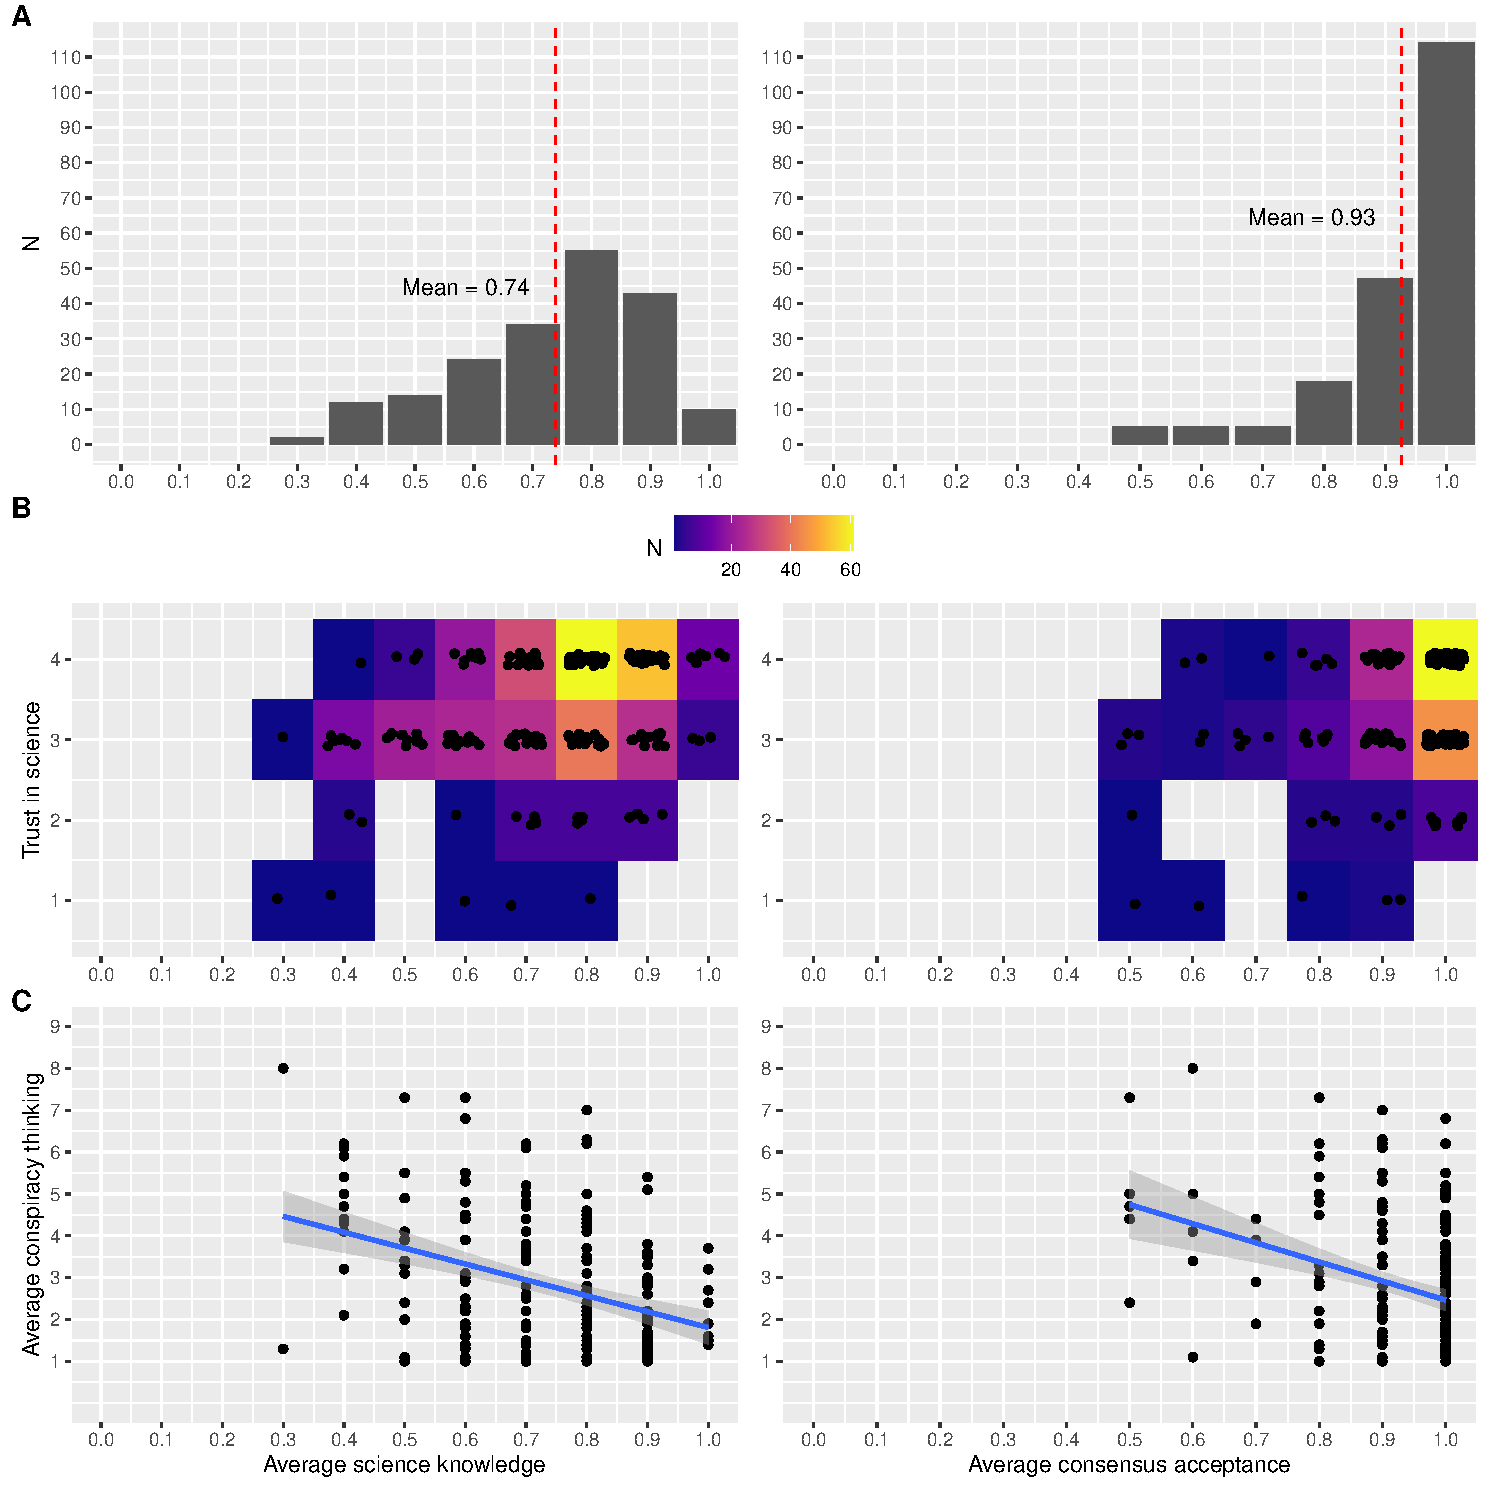
\includegraphics{output/figures/exp1-plot-overview.pdf}
\caption{\label{fig:exp1-plot-overview}Summary plot for Study 1. \textbf{A} Shows the distribution of science knowledge (left) and acceptance of scientific consensus \textbf{B} Shows the relationship between trust in science and science knowledge/acceptance of scientific consensus \textbf{C} Shows the relationship between conspiracy thinking and science knowledge/acceptance of scientific consensus}
\end{figure}

\clearpage

\section{Study 2}\label{exp2}

In study 1, we tested whether participants would accept the scientific consensus on basic science facts. In most instances they did, but not always. In study 2, we wanted to test whether this reluctance was because of participants not trusting us as a source of consensual science knowledge. To do so, we added an explanation and sources to each consensus statement, instead of only stating the consensus. To better understand reasons for consensus rejection, after having answered all questions, we asked participants an open-ended question to explain why they rejected the consensus, for each question on which they did so. We also excluded the where do trees their materials from, as this question clearly seemed to be an outlier where most participants would get the answer wrong.

Based on study 1, we formulated the following hypotheses:

\textbf{H1a: Higher trust in science is associated with more science knowledge?}

\textbf{H1b: Higher trust in science is associated with more acceptance of the scientific consensus, for participants who did not already know it?}

\textbf{H2a: Higher conspiracy thinking is associated with less science knowledge?}

\textbf{H2b: Higher conspiracy thinking is associated with less acceptance of the scientific consensus, for participants who did not already know it?}

We had the following research questions:

\textbf{RQ1: What is the average science knowledge score?}

\textbf{RQ2: When a participant's answer does not match the consensus, how often do they change their mind and accept the consensus?}

\textbf{RQ3: What reasons do participants provide to justify their rejection of the scientific consensus?}

\subsection{Participants}\label{participants-2}

We recruited 201 participants from the US via prolific. 11 participants failed our attention check, resulting in a final sample of 190 participants (96 female, 94 male; \(age_\text{mean}\): 43.48, \(age_\text{sd}\): 12.25, \(age_\text{median}\): 42). Since we did not have any prior assumptions on effect sizes and our analyses were descriptive, we did not do a power analysis.

\subsection{Procedure}\label{procedure-1}

The procedure was the same as in study 1, with the difference that, instead of just stating the scientific consensus, participants were presented with a short explanation which we wrote, partly based on explanations generated by ChatGPT, and three links to authoritative sources supporting the answer (Fig. \ref{fig:exp2-stimulus-example}.

\subsection{Materials}\label{materials-3}

We relied on the same items as in study 1. The only difference was that we removed the question on trees.

\FloatBarrier



\begin{figure}

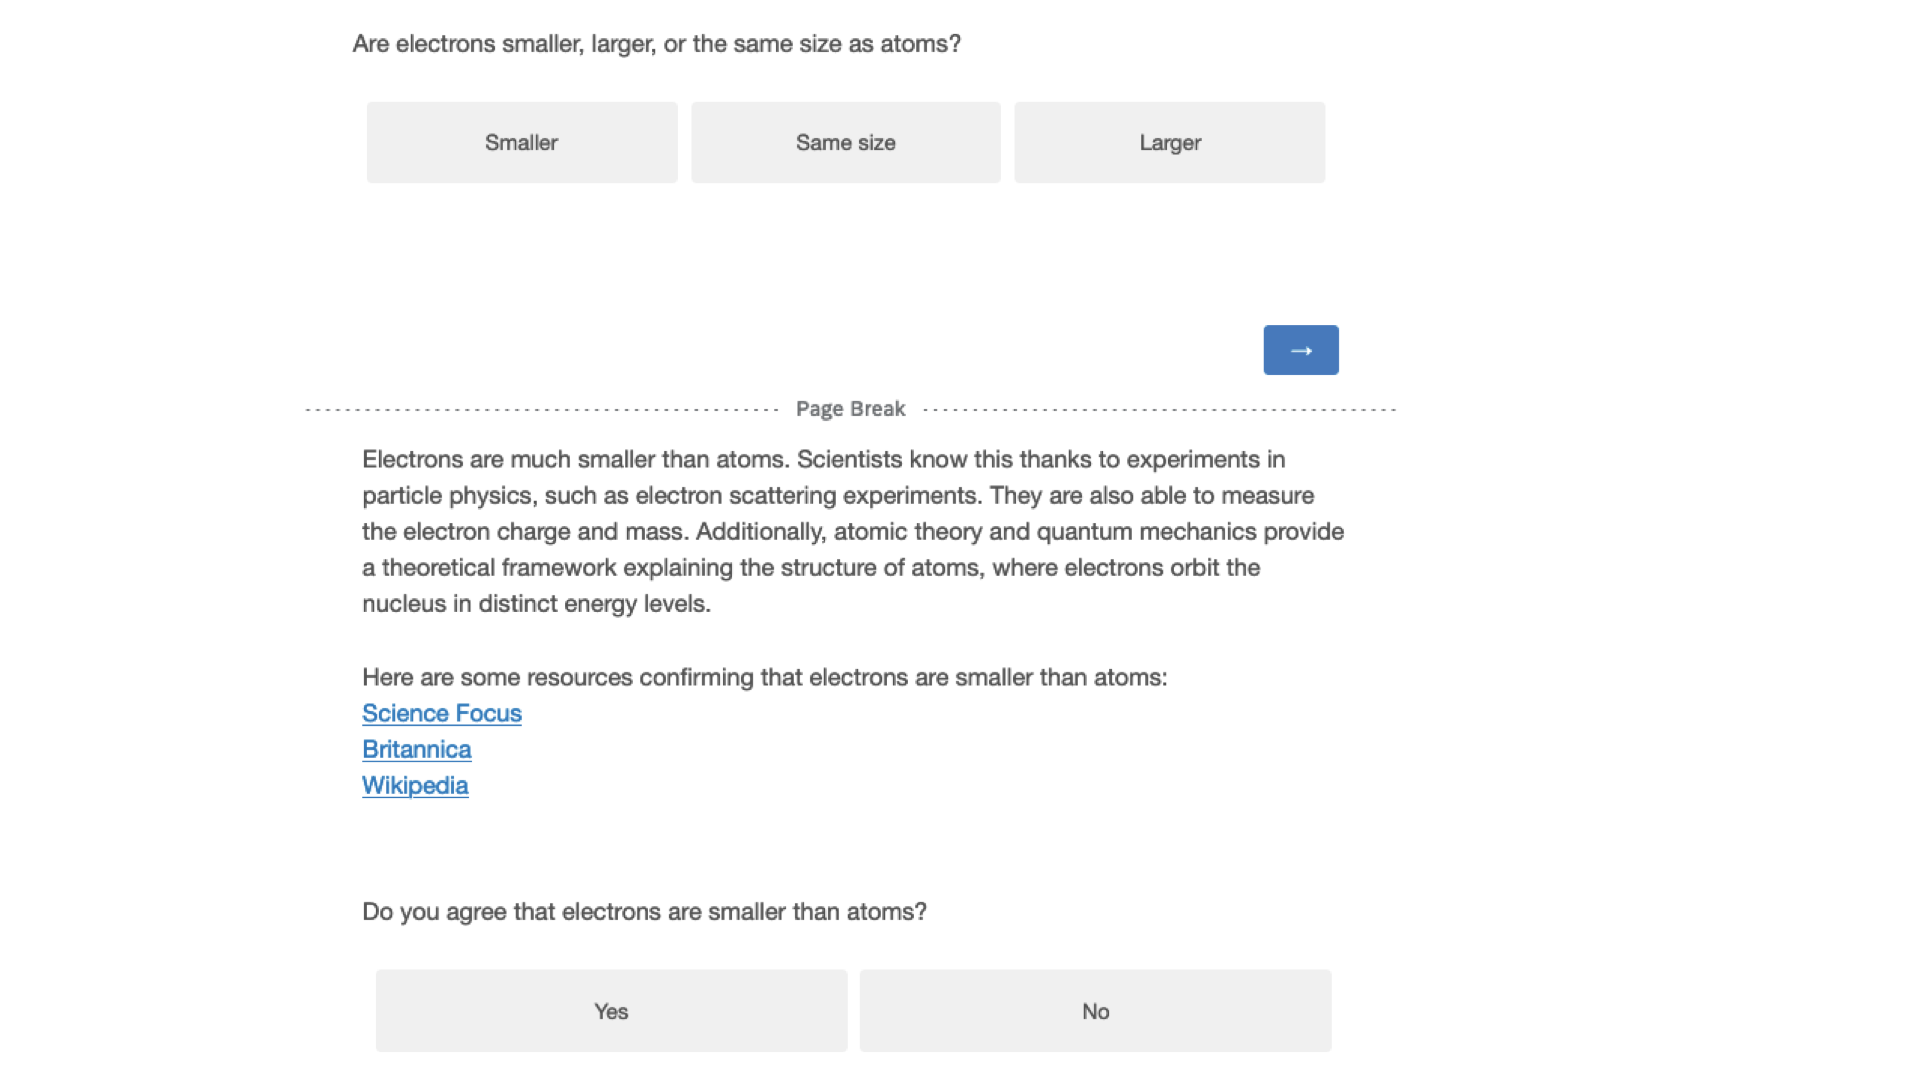
\includegraphics[width=1\linewidth]{./figures/study2_question_example} \hfill{}

\caption{Example of a science question, the scientific consensus and corresponding explanation and sources.}\label{fig:exp2-stimulus-example}
\end{figure}

\subsection{Results}\label{results-2}

As in study 1, we find a positive but small correlation between science knowledge and trust in science (H1a: r = 0.28, p \textless{} .001) and a small negative correlation between science knowledge and conspiracy thinking (H2a: r = -0.40, p \textless{} .001). By contrast to study 1, we conditioned on initially false answers when looking at the relationship of consensus acceptance with trust in science and conspiracy thinking, respectively. For trust in science, we find no statistically significant correlation (r = 0.16, p = 0.051). For conspiracy thinking we find a small negative one (r = -0.22, p = 0.006).

Confirming results from study 1, we find that the more people are knowledgeable about science and the more they tend to accept the scientific consensus even when they are not that knowledgeable in science, the more they tend to trust science. These correlations are relatively weak, which might be partly due to ceiling effects: (i) most people do trust science, and (ii) that is true even among people with low knowledge or acceptance rates. Below, we show that these results hold for our alternative measures of trust and conspiracy thinking. We also include more descriptive statistics, such as knowledge and acceptance by science questions.

Regarding RQ1, participants answered on average 79 \% (sd = 0.19) of the questions correctly, and accepted the scientific consensus on average for 98 \% (sd = 0.05) of the questions. In response to RQ2, in most cases (92.9 \%), participants readily accepted the scientific consensus after having initially given the wrong answer to a question. In very few cases (0.5 \%), participants who gave the correct response afterwards rejected the scientific consensus, thereby contradicting their own initial response.

\begin{table}[tbp]

\begin{center}
\begin{threeparttable}

\caption{\label{tab:exp2-justifications}Justifications by category}

\begin{tabular}{llll}
\toprule
Category & \multicolumn{1}{c}{N (instances)} & \multicolumn{1}{c}{Share (instances)} & \multicolumn{1}{c}{N (unique participants)}\\
\midrule
Personal convictions & 12.00 & 34.3\% & 8.00\\
Mistake & 9.00 & 25.7\% & 8.00\\
No justification & 7.00 & 20\% & 5.00\\
Not convinced & 5.00 & 14.3\% & 5.00\\
Religious Beliefs & 2.00 & 5.7\% & 2.00\\
\bottomrule
\end{tabular}

\end{threeparttable}
\end{center}

\end{table}

For RQ3, we got 35 answers from 25 different participants to the open-ended questions on why they had rejected the scientific consensus on a particular question. Table \ref{tab:exp2-justifications} summarizes these answers by five categories. All answers can be read in below.

\subsection{Discussion}\label{discussion-2}

Similar to study 1, most people (i) do know and agree with the scientific consensus, and (ii) tend to accept the scientific consent even if they were not previously aware of it (i.e.~answered the knowledge question wrongly). The share of these latter is considerably larger in study 2 (92.9 \%) than in study 1 (76.3 \%). While this could be just sampling variation, it might be that adding explanations and sources convinced people more than merely stating the consensus. We also show, again, that people with lower trust in science and who believe more in conspiracy theories tend to both know less about science and accept the scientific consensus less.

\subsection{Comparing items}\label{comparing-items-1}

\subsubsection{Conspiracy theories}\label{conspiracy-theories-1}

Table \ref{tab:exp2-correlation-conspiracy} shows the correlations of the three different scales assessing conspiracy thinking.

\begin{table}[h]

\begin{center}
\begin{threeparttable}

\caption{\label{tab:exp2-correlation-conspiracy}Correlations of the three different scales assessing conspiracy thinking}

\begin{tabular}{llll}
\toprule
 & \multicolumn{1}{c}{BCTI} & \multicolumn{1}{c}{CMQ} & \multicolumn{1}{c}{SICBS}\\
\midrule
BCTI & 1.00 & 0.66 & 0.63\\
CMQ & 0.66 & 1.00 & 0.86\\
SICBS & 0.63 & 0.86 & 1.00\\
\bottomrule
\end{tabular}

\end{threeparttable}
\end{center}

\end{table}

\subsubsection{Trust in science}\label{trust-in-science-2}

Table \ref{tab:exp2-correlation-trust} shows the correlations of the three different items measuring trust in science.

\begin{table}[h]

\begin{center}
\begin{threeparttable}

\caption{\label{tab:exp2-correlation-trust}Correlations of the three different items measuring trust in science}

\begin{tabular}{llll}
\toprule
 & \multicolumn{1}{c}{wgm\_sciencegeneral} & \multicolumn{1}{c}{wgm\_scientists} & \multicolumn{1}{c}{pew}\\
\midrule
wgm\_sciencegeneral & 1.00 & 0.89 & 0.79\\
wgm\_scientists & 0.89 & 1.00 & 0.85\\
pew & 0.79 & 0.85 & 1.00\\
\bottomrule
\end{tabular}

\end{threeparttable}
\end{center}

\end{table}

\subsection{Correlations with alternative measures}\label{correlations-with-alternative-measures-1}

Table \ref{tab:exp2-correlations-outcomes} shows the correlations between knowledge and acceptance, respectively, and outcome variables.

\begin{table}[tbp]

\begin{center}
\begin{threeparttable}

\caption{\label{tab:exp2-correlations-outcomes}Correlations between knowledge and acceptance, respectively, and outcome variables}

\begin{tabular}{lll}
\toprule
outcome & \multicolumn{1}{c}{Correlation with knowledge} & \multicolumn{1}{c}{Correlation with acceptance}\\
\midrule
BCTI (main conspiracy measure) & -0.4 (p< .001) & -0.37 (p< .001)\\
CMQ & -0.17 (p= 0.019) & -0.22 (p= 0.003)\\
SICBS & -0.14 (p= 0.058) & -0.2 (p= 0.006)\\
WGM trust scientists & 0.23 (p= 0.002) & 0.25 (p< .001)\\
WGM trust general (main trust measure) & 0.28 (p< .001) & 0.3 (p< .001)\\
PEW trust scientists & 0.16 (p= 0.027) & 0.22 (p= 0.003)\\
\bottomrule
\end{tabular}

\end{threeparttable}
\end{center}

\end{table}

\subsection{Results conditional on false responses}\label{results-conditional-on-false-responses-1}

Table \ref{tab:exp2-false-response-regression} shows the correlations between acceptance and outcome variables based on linear regression models on standardized values.

\begin{table}
\centering
\caption{\label{tab:exp2-false-response-regression}Based on false response data only, correlations between acceptance and outcome variables based on linear regression models on standardized values}
\centering
\begin{tabular}[t]{lcccccc}
\toprule
  & BCTI\_avg & CMQ\_avg & SICBS & wgm\_scientists & wgm\_sciencegeneral & pew\\
\midrule
(Intercept) & 0.000 & 0.000 & 0.000 & 0.000 & 0.000 & 0.000\\
 & (0.081) & (0.080) & (0.081) & (0.082) & (0.082) & \vphantom{1} (0.082)\\
avg\_acceptance & -0.225** & -0.247** & -0.201* & 0.131 & 0.161+ & 0.130\\
 & (0.081) & (0.080) & (0.081) & (0.082) & (0.082) & (0.082)\\
\midrule
Num.Obs. & 147 & 147 & 147 & 147 & 147 & 147\\
R2 & 0.051 & 0.061 & 0.041 & 0.017 & 0.026 & 0.017\\
R2 Adj. & 0.044 & 0.054 & 0.034 & 0.010 & 0.019 & 0.010\\
AIC & 414.5 & 412.9 & 416.1 & 419.6 & 418.3 & 419.7\\
BIC & 423.5 & 421.9 & 425.0 & 428.6 & 427.3 & 428.6\\
Log.Lik. & -204.248 & -203.465 & -205.036 & -206.802 & -206.141 & -206.826\\
RMSE & 0.97 & 0.97 & 0.98 & 0.99 & 0.98 & 0.99\\
\bottomrule
\multicolumn{7}{l}{\rule{0pt}{1em}+ p $<$ 0.1, * p $<$ 0.05, ** p $<$ 0.01, *** p $<$ 0.001}\\
\end{tabular}
\end{table}



\begin{figure}
\centering
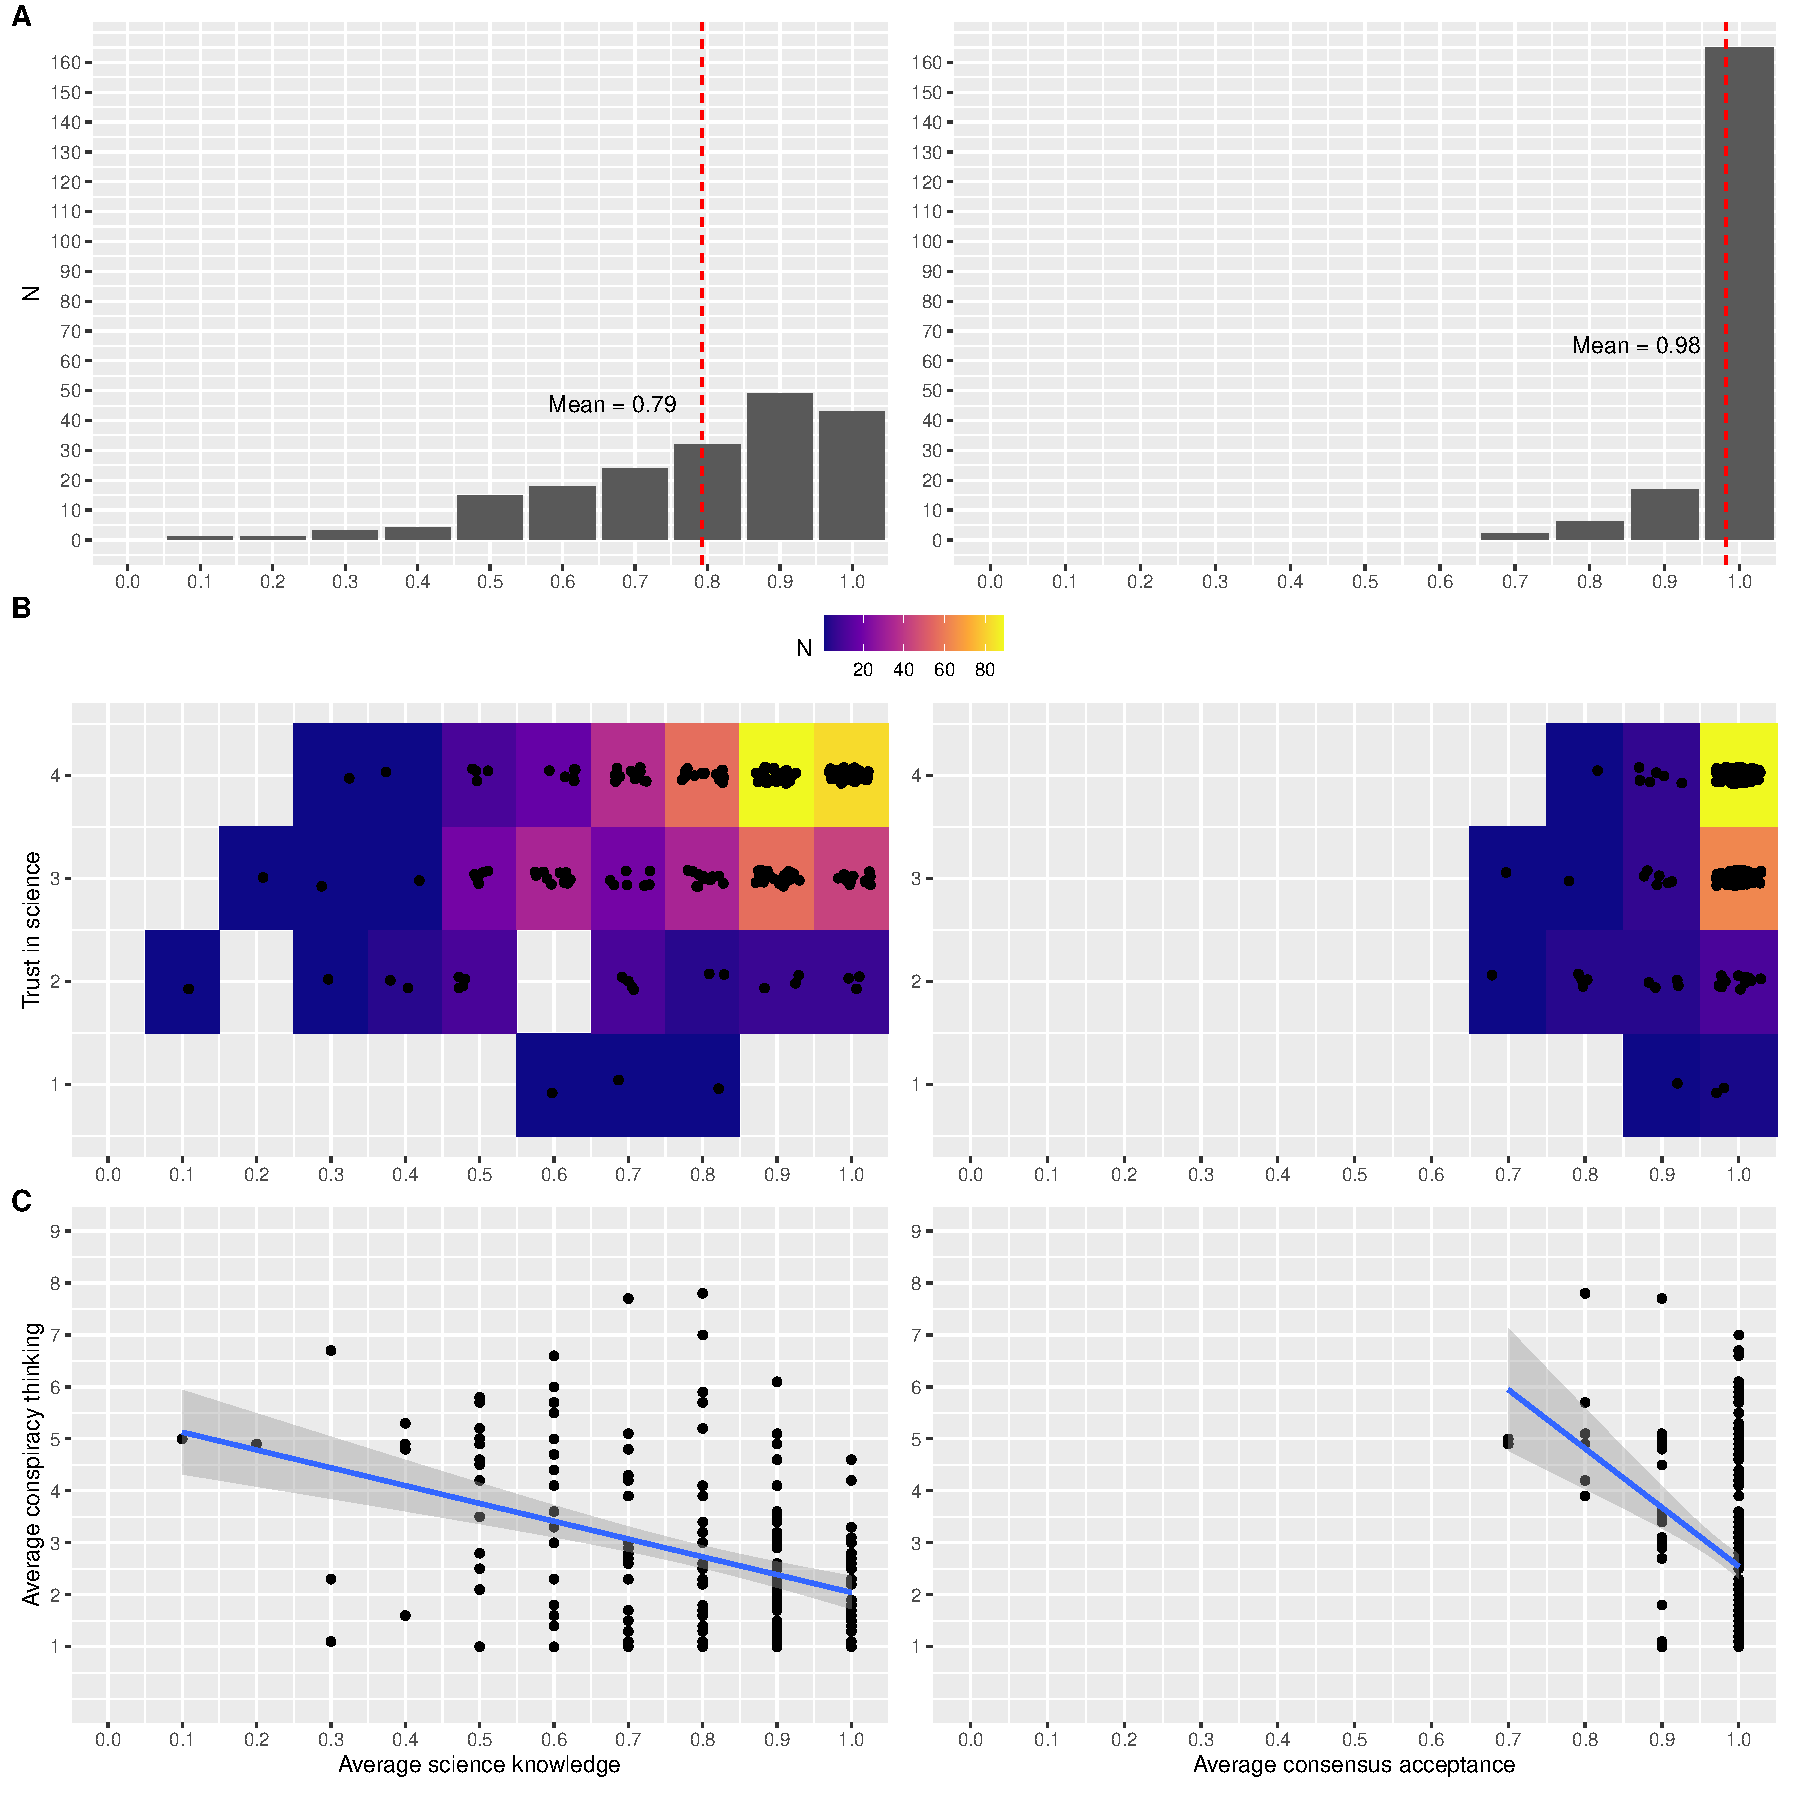
\includegraphics{output/figures/exp2-plot-overview.pdf}
\caption{\label{fig:exp2-plot-overview}Summary plot for Study 2. \textbf{A} Shows the distribution of science knowledge (left) and acceptance of scientific consensus for participants who gave the wrong answer \textbf{B} Shows the relationship between trust in science and science knowledge/acceptance (if wrong at first, rounded to the first digit) of scientific consensus \textbf{C} Shows the relationship between conspiracy thinking and science knowledge/acceptance (if wrong at first) of scientific consensus}
\end{figure}

\clearpage

\section{Study 3}\label{exp3}

Study 3 is essentially a replication-\/--with some minor modifications-\/--of study 2, but on a different type of sample. Both study 1 and 2 were run on convenience samples. For study 3, we recruited a sample of people holding anti-vaccination beliefs (see below). By contrast to study 2, after asking participants an open question about why they did not accept the consensus (in cases where they didn't), we provide them with an explicit opportunity to change their answer (Fig. \ref{fig:exp3-explanation-example}). Based on the answers to the open-ended questions, we also pre-registered a categorization scheme of reasons why people rejected the consensus. Finally, we also ask participants about why they agree with the scientific consensus on certain questions, in case they do. We want to know if participants perceive that this is because of trust, or other factors.

As for study 2 (but without conditioning on wrong answers, as we did in study 1), we had the following hypotheses:

\textbf{H1a: Higher trust in science is associated with more science knowledge?}

\textbf{H1b: Higher trust in science is associated with more acceptance of the scientific consensus.}

\textbf{H2a: Higher conspiracy thinking is associated with less science knowledge?}

\textbf{H2b: Higher conspiracy thinking is associated with less acceptance of the scientific consensus.}

We had the following research questions:

\textbf{RQ1: What is the average science knowledge score?}

\textbf{RQ2: What is the average acceptance of the scientific consensus}

\textbf{RQ3: What reasons do participants provide to justify their rejection of the scientific consensus?}

\textbf{RQ4: In case they agree with the scientific consensus, do people feel that this is because of trust?}

\subsection{Participants}\label{participants-3}

We recruited a sample of participants holing vaccine-skeptic beliefs. Prolific Academic allows to filter out participants who have given specific answers to certain questions. We selected three available questions: 1. ``Participants were asked the following question: Please describe your attitudes towards the COVID-19 (Coronavirus) vaccines: {[}For (I feel positively about the vaccines); Against (I feel negatively about the vaccines); Neutral (I don't have strong opinions either way); Prefer not to say''{]}. We selected particpants who answered''Against''. 2. ``Participants were asked the following question: Have you received a coronavirus (COVID-19) vaccination? {[}Yes (at least one dose); No; Prefer not to answer{]}''. We select only people who answered ``No''. 3. ``Participants were asked the following question: On a scale from 1-7, please rate to what extent you agree with the following statement: I believe that scheduled immunizations are safe for children. {[}1 (TOTALLY DISAGREEE); 2 (DISAGREE); 3 (SOMEWHAT DISAGREE); 4 (NEITHER AGREE NOR DISAGREE); 5 (SOMEWHAT AGREE); 6 (AGREE); 7 (TOTALLY AGREE); Rather not say''{]}. We select only people who answered''1'', ``2'', or ``3''.

Based on these criteria, we recruited 200 participants from the US via prolific, of which none failed our attention check, resulting in a final sample of 200 participants (125 female, 73 male; \(age_\text{mean}\): 42.90, \(age_\text{sd}\): 12.00, \(age_\text{median}\): 41). Since we did not have any prior assumptions on effect sizes and our analyses were descriptive, we did not do a power analysis.

However, due to a randomization mistake for our outcomes, participant answered only two of the three outcome measure blocs (trust in science, conspiracy thinking, and reason for accepting consensus). This leaves us with reduced sample sizes for all analyses concerning these outcomes (N = 140 for trust in science, N = 138 for conspiracy measures, N = 122 for reason for accepting consensus).

\subsection{Procedure}\label{procedure-2}

The procedure was mostly the same as in study 2. In addition, after each open-ended question on cases where participants rejected the scientific consensus, participants were also asked if they want to change their answer and accept the scientific consensus. Finally, at the end of the survey, we asked participants: ``For the questions in which you agreed with the scientific consensus, would you say that\ldots?'' The answer options were: (i) ``You mostly agree with the consensus because, on that question, you trust scientists'', (ii) ``You mostly agree with the consensus because you have been able to independently verify it'', and (iii) ``Other'', with a text box for participants to explain. Participants who selected ``You mostly agree with the consensus because you have been able to independently verify it'', were asked the open-ended follow-up question: ``Could you please tell us how you independently verified the information?''.

\subsection{Materials}\label{materials-4}

\FloatBarrier



\begin{figure}

{\centering 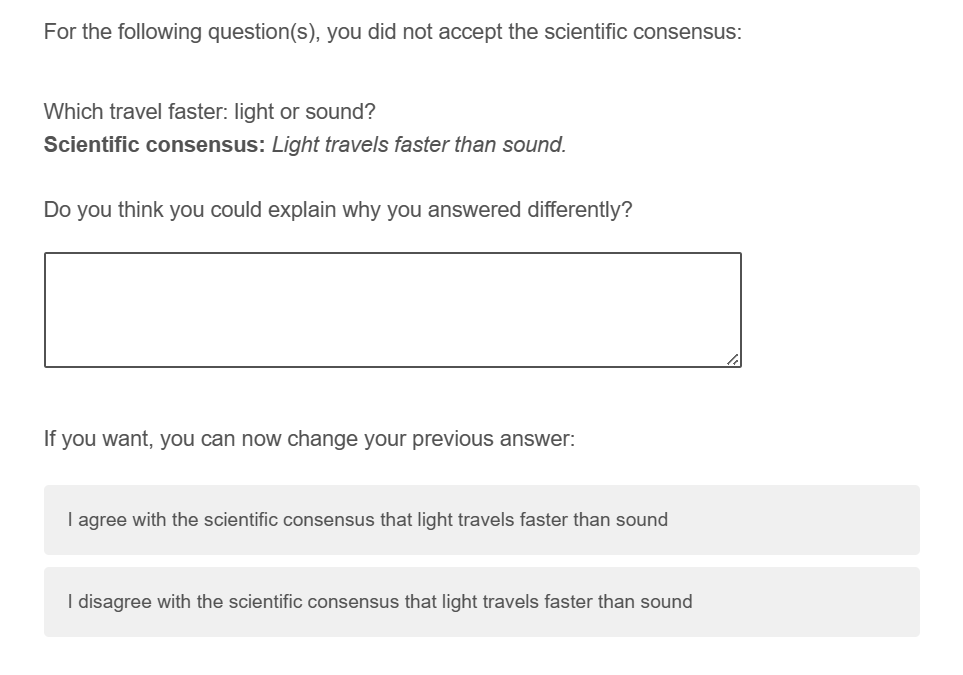
\includegraphics[width=0.5\linewidth]{figures/study3_example_explanation} 

}

\caption{Example of an explanation question and the opportunity to change the previous answer.}\label{fig:exp3-explanation-example}
\end{figure}

Table \ref{tab:exp3-knowledge-items} shows all questions, their scientifically consensual answer, and their source. All but two questions were selected from existing science knowledge questionnaires. We tried to select non-political questions.

\begingroup\fontsize{8}{10}\selectfont

\begin{longtable}[t]{>{\raggedleft\arraybackslash}p{1em}>{\raggedright\arraybackslash}p{10em}>{\raggedright\arraybackslash}p{10em}>{\raggedright\arraybackslash}p{23em}}
\caption{\label{tab:exp3-knowledge-items}Science knowledge items}\\
\toprule
id & Question & Scientific consensus (Study 1) & Explanation (Study 2 \& 3)\\
\midrule
1 & Do antibiotics kill viruses as well as bacteria? & There is a consensus among scientists that antibiotics kill bacteria, but not viruses. & Antibiotics specifically target and kill bacteria, not viruses. Scientists know this thanks to extensive laboratory experiments and clinical trials where antibiotics have been observed to be effective against bacterial infections but not viral ones. Scientists have also studied how antibiotics work, which typically involve disrupting bacterial cell processes like cell wall synthesis or protein production, which are absent in viruses.

Here are some resources confirming that antibiotics only kill bacteria: 
American Chemical Society
Queensland Government 
Wikipedia\\
2 & Are electrons smaller, larger, or the same size as atoms ? & There is a consensus among scientists that electrons are smaller than atoms. & Electrons are much smaller than atoms. Scientists know this thanks to experiments in particle physics, such as electron scattering experiments. They are also able to measure the electron charge and mass. Additionally, atomic theory and quantum mechanics provide a theoretical framework explaining the structure of atoms, where electrons orbit the nucleus in distinct energy levels.

Here are some resources confirming that electrons are smaller than atoms:
Science Focus 
Britannica 
Wikipedia\\
3 & Have the continents on Earth been moving for millions of years or have they always been where they are now? & There is a consensus among scientists that the continents on Earth have been moving for millions of years due to plate tectonics. & The continents on Earth have been moving for millions of years due to plate tectonics. Scientists have gathered evidence from various sources, including fossil records, geological formations, and the magnetic properties of rocks. The theory of plate tectonics explains how the Earth's lithosphere is divided into large, rigid plates that move over the semi-fluid asthenosphere, leading to phenomena like continental drift, earthquakes, and volcanic activity.

Here are some resources confirming that continents on Earth have been moving for millions years:
Britannica 
Live Science 
National Geographic\\
4 & What decides whether a baby is a boy or a girl ? Is it the father’s genes, the mother’s genes, or both? & There is a consensus among scientists that it is the genes in the father's sperm which are decisive on whether a baby is a boy or a girl. & Chromosomes are structures found in the nucleus of cells that carry long pieces of DNA. Two of the chromosomes (the X and the Y chromosome) are called sex chromosomes. In most cases, females have two X chromosomes, while males have one X and one Y chromosome. At conception, the mother transmits an X chromosome, and the father may contribute an X or a Y. The chromosome from the father therefore determines if the baby is female (if the father transmits an X) or male (if the father transmits a Y). In most cases, children are born a male or female according to their chromosomes. However, some children may be born with genitalia that do not match their chromosomes.

Here are some resources confirming that it is the father's genes that decide the sex of a baby: 
National Library of Medicine 
Nature 
Wikipedia\\
5 & Do lasers work by focusing sound waves? & There is a consensus among scientists that lasers do not work by focusing sound waves. & Lasers produce a narrow beam of light in which all of the particles of light have very similar wavelengths. The laser’s lightwaves travel together with their peaks all lined up, in phase. This is why laser beams are very narrow, very bright, and can be focused into a very tiny spot. Because laser light stays focused and does not spread out much (like a flashlight would), laser beams can travel very long distances.

Here are some resources confirming that lasers do not work by focusing sound waves: 
NASA 
Lawrence Livermore National Library
Wikipedia\\
\addlinespace
6 & How long does it take for Earth to go around the sun: one day, one month, or one year ? & There is a consensus among scientists that it takes one year for Earth to go around the sun. & Earth takes approximately one year to orbit the sun. This knowledge is based on astronomical observations and measurements of celestial motion. Early astronomers tracked the movement of the Earth relative to the stars and planets, leading to the development of models that accurately predict the Earth's orbital period around the sun.

Here are some resources confirming that Earth goes around the sun in one year: 
NASA
National Geographic 
Wikipedia\\
7 & Are diamonds made of carbon ? & There is a consensus among scientists that diamonds are made of carbon. & Diamonds are made of only one element, carbon. Carbon is the same element that makes coal or graphite used for pencils. Why are diamonds transparent and hard while coal and graphite are opaque and soft? It all comes down to the placement of their atoms. In diamonds, each carbon atom is bonded to 4 other carbon atoms, while in graphite, each atom is only bonded to 3 other carbon atoms. The bonds in diamonds are held in such a tight structure that all light passes around them, which is why diamonds look transparent. In coal and graphite, light gets trapped between the atoms, which is why they look dark and opaque. Why do carbon atoms bond differently in diamonds? At very high pressures and temperatures, the carbon atoms are squeezed so much that they start touching more atoms. When the pressure is about 50,000 times the pressure at the surface of the Earth and the temperature is about 1600°C, the carbon atoms bond with 4 other atoms and result in diamonds.

Here are some resources confirming that diamonds are made of carbon: 
Arizona State University 
University of Bristol 
Wikipedia\\
8 & Which travels faster : light or sound? & There is a consensus among scientists that light travels faster than sound. & Light travels faster than sound. This conclusion arises from numerous experiments and observations in physics. You can also experience this for yourself during a thunderstorm. Unless the lighting is right above you, you will first see the lighting, then hear the thunder some time after (you can even tell how far the lighting struck by counting how many seconds it takes for the thunder to reach you). More precisely, the speed of light has been measured accurately using techniques such as the Michelson–Morley experiment. Similarly, the speed of sound has been measured through experiments involving the propagation of sound waves through various materials.

Here are some resources confirming that light travers faster than sound: 
NASA 
Wikipedia : Speed of light 
Wikipedia: Speed of sound\\
9 & Is common table salt made of calcium carbonate? & There is a consensus among scientists that common table salt is not made of calcium carbonate; it is made of sodium chloride. & Common table salt, or sodium chloride (NaCl), is not made of calcium carbonate. Scientists can use a variety of tests to understand what matter is made of. The most used test for sodium chloride is the chemical reaction with silver nitrate. The presence of sodium chloride yields a white precipitate upon drops of a silver nitrate solution. Calcium carbonate, by contrast, is the substance that makes up, for instance, chalk.

Here are some resources confirming that common table salt is not made of calcium carbonate: 
National Library of Medicine 
Chem Europe 
Wikipedia\\
10 & Is water made of molecules containing one oxygen and two hydrogen atoms? & There is a consensus among scientists that water is made of molecules containing one oxygen and two hydrogen atoms, and that its chemical formula is therefore H2O. & Water is made of molecules containing one oxygen atom and two hydrogen atoms, chemically represented as H2O. We know this for instance because if you set hydrogen on fire in a container with oxygen, water will form on the sides of the container. More recent techniques such as spectroscopy and X-ray crystallography have allowed scientists to more directly see the composition and structure of water molecules, confirming the presence of two hydrogen atoms bonded to one oxygen atom.

Here are some resources confirming that water is made of molecules containing one oxygen and two hydrogen atoms:
National Library of Medicine 
Wikipedia: Chemical structure 
Wikipedia: Water\\
\addlinespace
11 & Where do trees mainly draw the materials with which they create their mass? & There is a consensus among scientists that carbon drawn from the air during photosynthesis makes up most of the materials that trees use to build new leaves, stems, and roots. & \\
\bottomrule
\end{longtable}
\endgroup{}

\subsection{Results}\label{results-3}

As in study 1 and 2, we find that participants answered on average 75 \% (sd = 0.18) of the questions correctly (RQ1), and initially accepted the scientific consensus on average for 96 \% (sd = 0.08) of the questions (RQ2). The acceptance rate is even higher when accounting for opinion revisions towards acceptance of the consensus, after initial rejection (98 \%, sd = 0.06).

In most cases (87 \%), participants readily accepted the scientific consensus right after having given the wrong answer to a question. After providing the chance to revise the initial consensus rejection, this share is even larger (95.5 \%). In very few cases (0.9 \%), participants who initially gave the correct response afterwards rejected the scientific consensus right after, thereby contradicting their own initial response. This share drops slightly after providing the chance to revise the initial consensus rejection (0.7 \%).

For all correlations, we include opinion revisions for measuring consensus acceptance. We find no statistically significant correlation between science knowledge and trust in science (r = 0.14, p = 0.100), but a samll positive correlation between acceptance of scientific consensus and trust in science (r = 0.20, p = 0.019). Again, these findings might be partly due to ceiling effects: (i) most people do trust science, and (ii) that is true even among people with low knowledge or acceptance rates. We find no statistically significant correlation between conspiracy thinking and science knowledge (r = -0.16, p = 0.055), and between conspiracy thinking and acceptance of scientific consensus (r = -0.02, p = 0.788).

For RQ3, we got 74 answers from 47 different participants to the open-ended questions on why they had rejected the scientific consensus on a particular question. Table \ref{tab:exp3-justifications} summarizes these answers by five categories.

All answers can be read in the below.

\begin{table}[tbp]

\begin{center}
\begin{threeparttable}

\caption{\label{tab:exp3-justifications}Justifications by category}

\begin{tabular}{llll}
\toprule
Category & \multicolumn{1}{c}{N (instances)} & \multicolumn{1}{c}{Share (instances)} & \multicolumn{1}{c}{N (unique participants)}\\
\midrule
Personal convictions & 25.00 & 33.8\% & 19.00\\
Mistake & 21.00 & 28.4\% & 18.00\\
No justification & 18.00 & 24.3\% & 13.00\\
Not convinced & 7.00 & 9.5\% & 3.00\\
Religious Beliefs & 3.00 & 4.1\% & 3.00\\
\bottomrule
\end{tabular}

\end{threeparttable}
\end{center}

\end{table}

For RQ4, we had 122 participants answering the question. Of these 41.8\% said they accepted the scientific consensus because they trust scientists on this question, while 47.5\% said they independently verified the fact. 10.7\% answered with other ``other'' and gave an open-ended explanation (see below for all open-ended answers).

We also asked all 58 participants who answered that they had independently verified the answer to explain how they did so. The open-ended answers are listed below.

\subsection{Comparing items}\label{comparing-items-2}

\subsubsection{Conspiracy theories}\label{conspiracy-theories-2}

Table \ref{tab:exp3-correlation-conspiracy} shows the correlations of the three different scales assessing conspiracy thinking.

\begin{table}[h]

\begin{center}
\begin{threeparttable}

\caption{\label{tab:exp3-correlation-conspiracy}Correlations of the three different scales assessing conspiracy thinking}

\begin{tabular}{llll}
\toprule
 & \multicolumn{1}{c}{BCTI} & \multicolumn{1}{c}{CMQ} & \multicolumn{1}{c}{SICBS}\\
\midrule
BCTI & 1.00 & NA & NA\\
CMQ & NA & 1.00 & NA\\
SICBS & NA & NA & 1.00\\
\bottomrule
\end{tabular}

\end{threeparttable}
\end{center}

\end{table}

\subsubsection{Trust in science}\label{trust-in-science-3}

Table \ref{tab:exp3-correlation-trust} shows the correlations of the three different items measuring trust in science.

\begin{table}[h]

\begin{center}
\begin{threeparttable}

\caption{\label{tab:exp3-correlation-trust}Correlations of the three different items measuring trust in science}

\begin{tabular}{llll}
\toprule
 & \multicolumn{1}{c}{wgm\_sciencegeneral} & \multicolumn{1}{c}{wgm\_scientists} & \multicolumn{1}{c}{pew}\\
\midrule
wgm\_sciencegeneral & 1.00 & 0.77 & 0.68\\
wgm\_scientists & 0.77 & 1.00 & 0.68\\
pew & 0.68 & 0.68 & 1.00\\
\bottomrule
\end{tabular}

\end{threeparttable}
\end{center}

\end{table}

\subsection{Correlations with alternative measures}\label{correlations-with-alternative-measures-2}

Table \ref{tab:exp3-correlations-outcomes} shows the correlations between knowledge and acceptance, respectively, and outcome variables.

\begin{table}[tbp]

\begin{center}
\begin{threeparttable}

\caption{\label{tab:exp3-correlations-outcomes}Correlations between knowledge and acceptance, respectively, and outcome variables}

\begin{tabular}{lll}
\toprule
outcome & \multicolumn{1}{c}{Correlation with knowledge} & \multicolumn{1}{c}{Correlation with acceptance}\\
\midrule
BCTI (main conspiracy measure) & -0.16 (p= 0.055) & -0.03 (p= 0.788)\\
CMQ & 0.01 (p= 0.925) & -0.01 (p= 0.934)\\
SICBS & 0.02 (p= 0.767) & 0 (p= 0.987)\\
WGM trust scientists & 0.11 (p= 0.193) & 0.2 (p= 0.007)\\
WGM trust general (main trust measure) & 0.14 (p= 0.100) & 0.17 (p= 0.019)\\
PEW trust scientists & -0.08 (p= 0.367) & 0.12 (p= 0.104)\\
\bottomrule
\end{tabular}

\end{threeparttable}
\end{center}

\end{table}

\subsection{Results conditional on false responses}\label{results-conditional-on-false-responses-2}

Table \ref{tab:exp3-false-response-regression} shows the correlations between acceptance and outcome variables based on linear regression models on standardized values.

\begin{table}
\centering
\caption{\label{tab:exp3-false-response-regression}Based on false response data only, correlations between acceptance and outcome variables based on linear regression models on standardized values}
\centering
\begin{tabular}[t]{lcccccc}
\toprule
  & BCTI\_avg & CMQ\_avg & SICBS & wgm\_scientists & wgm\_sciencegeneral & pew\\
\midrule
(Intercept) & -0.001 & 0.000 & 0.000 & 0.005 & 0.002 & 0.008\\
 & (0.091) & (0.091) & (0.091) & (0.088) & (0.089) & (0.088)\\
avg\_acceptance & -0.043 & -0.025 & -0.009 & 0.083 & 0.039 & 0.125\\
 & (0.090) & (0.090) & (0.090) & (0.079) & (0.079) & (0.078)\\
\midrule
Num.Obs. & 122 & 122 & 122 & 128 & 128 & 128\\
R2 & 0.002 & 0.001 & 0.000 & 0.009 & 0.002 & 0.020\\
R2 Adj. & -0.006 & -0.008 & -0.008 & 0.001 & -0.006 & 0.012\\
AIC & 351.0 & 351.1 & 351.2 & 367.1 & 368.0 & 365.7\\
BIC & 359.4 & 359.6 & 359.6 & 375.7 & 376.5 & 374.2\\
Log.Lik. & -172.491 & -172.571 & -172.604 & -180.560 & -180.996 & -179.843\\
RMSE & 0.99 & 1.00 & 1.00 & 0.99 & 1.00 & 0.99\\
\bottomrule
\multicolumn{7}{l}{\rule{0pt}{1em}+ p $<$ 0.1, * p $<$ 0.05, ** p $<$ 0.01, *** p $<$ 0.001}\\
\end{tabular}
\end{table}



\begin{figure}
\centering
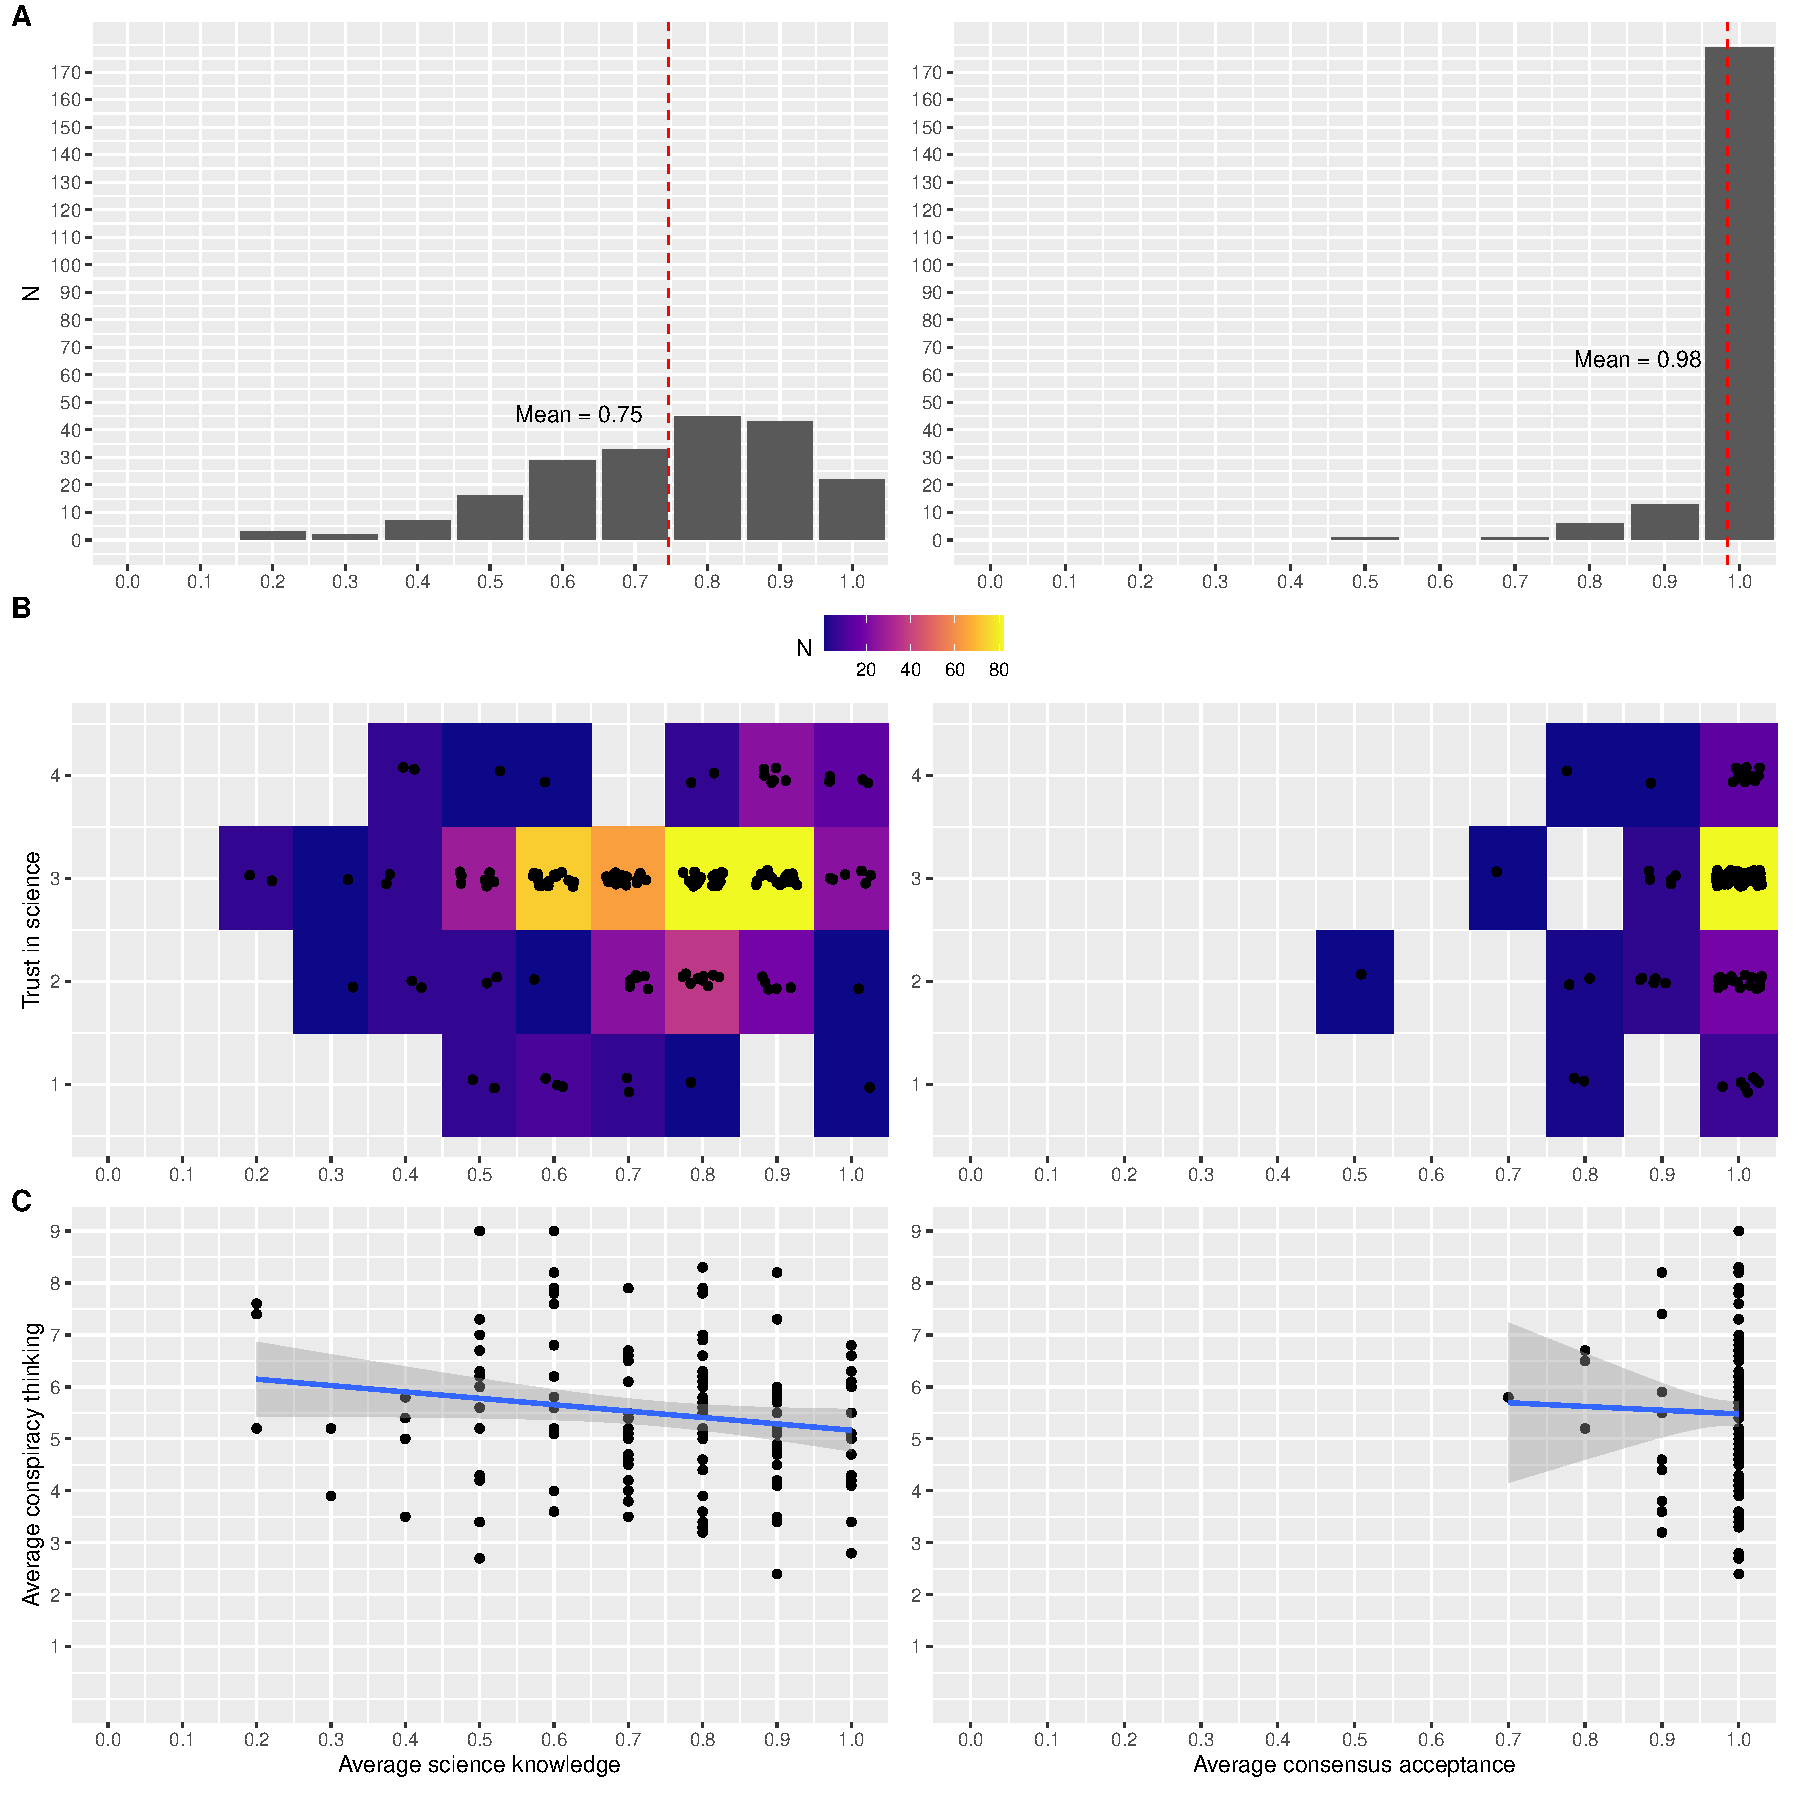
\includegraphics{output/figures/exp3-plot-overview.pdf}
\caption{\label{fig:exp3-plot-overview}Summary plot for Study 3. \textbf{A} Shows the distribution of science knowledge (left) and acceptance of scientific consensus for participants who gave the wrong answer \textbf{B} Shows the relationship between trust in science and science knowledge/acceptance (if wrong at first, rounded to the first digit) of scientific consensus \textbf{C} Shows the relationship between conspiracy thinking and science knowledge/acceptance (if wrong at first) of scientific consensus}
\end{figure}

\clearpage

\section{Study 4}\label{exp4}

Study 4 relies on broadly the same design as study 3, and is again run on a sample of participants with vaccine-skeptic beliefs. The main difference is that study 4 uses a set of science questions which, instead of being on well-established facts, we are about more recent discoveries (Table \ref{tab:exp4-knowledge}). Our main question is whether participants will nevertheless readily accept the scientific consensus, as they did for the basic facts in previous studies.

As for the previous studies, we had the following hypotheses:

\textbf{H1a: Higher trust in science is associated with more science knowledge?}

\textbf{H1b: Higher trust in science is associated with more acceptance of the scientific consensus.}

\textbf{H2a: Higher conspiracy thinking is associated with less science knowledge?}

\textbf{H2b: Higher conspiracy thinking is associated with less acceptance of the scientific consensus.}

We had the following research questions:

\textbf{RQ1: What is the average science knowledge score?}

\textbf{RQ2: What is the average acceptance of the scientific consensus}

\textbf{RQ3: What reasons do participants provide to justify their rejection of the scientific consensus?}

\textbf{RQ4: In case they agree with the scientific consensus, do people feel that this is because of trust?}

\subsection{Participants}\label{participants-4}

We recruited a sample of participants holing vaccine-skeptic beliefs. Prolific Academic allows to filter out participants who have given specific answers to certain questions. We selected three available questions: 1. ``Participants were asked the following question: Please describe your attitudes towards the COVID-19 (Coronavirus) vaccines: {[}For (I feel positively about the vaccines); Against (I feel negatively about the vaccines); Neutral (I don't have strong opinions either way); Prefer not to say''{]}. We selected particpants who answered''Against''. 2. ``Participants were asked the following question: Have you received a coronavirus (COVID-19) vaccination? {[}Yes (at least one dose); No; Prefer not to answer{]}''. We select only people who answered ``No''. 3. ``Participants were asked the following question: On a scale from 1-7, please rate to what extent you agree with the following statement: I believe that scheduled immunizations are safe for children. {[}1 (TOTALLY DISAGREEE); 2 (DISAGREE); 3 (SOMEWHAT DISAGREE); 4 (NEITHER AGREE NOR DISAGREE); 5 (SOMEWHAT AGREE); 6 (AGREE); 7 (TOTALLY AGREE); Rather not say''{]}. We select only people who answered''1'', ``2'', or ``3''.

Based on these criteria, we recruited 200 participants from the US via prolific, of which two failed our attention check, resulting in a final sample of 198 participants (98 female, 100 male; \(age_\text{mean}\): 42.67, \(age_\text{sd}\): 12.32, \(age_\text{median}\): 41). Since we did not have any prior assumptions on effect sizes and our analyses were descriptive, we did not do a power analysis.

\subsection{Procedure}\label{procedure-3}

The procedure was identical to the one in study 3.

\subsection{Materials}\label{materials-5}

\FloatBarrier

Table \ref{tab:exp4-knowledge} shows all questions, their scientifically consensual answer, and their source. All but two questions were selected from existing science knowledge questionnaires. We tried to select non-political questions.

\begingroup\fontsize{8}{10}\selectfont

\begin{longtable}[t]{>{\raggedleft\arraybackslash}p{1em}>{\raggedright\arraybackslash}p{12em}>{\raggedright\arraybackslash}p{10em}>{\raggedright\arraybackslash}p{12em}}
\caption{\label{tab:exp4-knowledge}Science knowledge items}\\
\toprule
id & Question & Scientific consensus & Sources\\
\midrule
1 & For which disease is the drug bedaquiline, developed in 2007, a treatment? [Tetanus; Tuberculosis; Malaria] & There is a consensus among scientists that the drug bedaquiline is used against tubercolisis. & Sources: Wikipedia: https://en.wikipedia.org/wiki/Bedaquiline ;  Journal of applied microbiology: https://enviromicro-journals.onlinelibrary.wiley.com/doi/full/10.1111/jam.14478\#:\textasciitilde{}:text=The\%20drug\%20bedaquiline\%20was\%20approved,\%2DTB\%20and\%20XDR\%2DTB\\
2 & What is the maximum speed a proton can attain in the largest particle collider as to 2015? [90\% of the speed of light; 99\% of the speed of light; the speed of light] & There is a consensus among scientists that the maximum speed a proton can attain in the largest particle collider (the Large Hadron Collider) is 99\% of the speed of light. & Sources: Wikipedia: https://en.wikipedia.org/wiki/Large\_Hadron\_Collider\#Findings\_and\_discoveries ; CERN: https://home.cern/news/news/accelerators/first-successful-beam-record-energy-65-tev\\
3 & Kepler-452b is an exoplanet revolving around the star Kepler-452. How far away from the star is it, as established by astronomers in 2015? [97 million mi; 1,2 million mi; 1254 million mi] & There is a consensus among scientists that Kepler-452b is 97 million mi away from its star Kepler-452. & Wikipedia: https://en.wikipedia.org/wiki/Kepler-452b; NASA: https://science.nasa.gov/exoplanet-catalog/kepler-452-b/\\
4 & Using bomb-pusle dating with carbon 14, what is the age of the oldest known vertebrate, as established in 2016? [138 years; 205 years;  392 years] & There is a consensus among scientists that the oldest known vertebrate in 2016 was 392 years old, it is the Greenland shark. & Sources:  Wikipedia: https://en.wikipedia.org/wiki/Bomb\_pulse\#Applications Oxford University Research Archive: https://ora.ox.ac.uk/objects/uuid:6c040460-9519-4720-9669-9911bdd03b09\\
5 & How many more glials cells are there in the brain in comparison with neurons, as established in 2016? [The same amount; Twice as many; Tenth as many] & There is a consensus among scientists that there is the same amount of glial cells and neurons in the brain. & Sources: The Journal of Comparative neurology: https://onlinelibrary.wiley.com/doi/10.1002/cne.24040; Wikipedia: https://en.wikipedia.org/wiki/Glia\#Total\_number\\
\addlinespace
6 & As predicted by the general theory of relativity, how many times would the Earth keep orbiting if the Sun disappeared, as established in 2012? [47 seconds; 8 minutes;  2 hours] & There is a consensus among scientists that if the Sun disappeared, the Earth would keep orbiting for 8 minutes. & Sources: Wikipedia: https://en.wikipedia.org/wiki/Gravity\#Tests\_of\_general\_relativity ; Science Bulletin: https://link.springer.com/article/10.1007/s11434-012-5603-3\\
7 & What is the electric charge of the Higgs Boson, as established in 2012? [1.602176634 x 10-19; 0; 3.2x10-19C] & There is a consensus among scientists that the Higgs Boson does not have an electric charge, it is electrically neutral. & Sources: Wikipedia: https://en.wikipedia.org/wiki/Higgs\_boson\#cite\_ref-npr-interview\_189-0; Cern: https://home.cern/science/physics/higgs-boson\\
8 & What is the age of the oldest materials formed on Earth, as established in 2020? [Less than 4.6 Ga; Around 4.6 Ga; More than 4.6 Ga] & There is a consensus among scientists that the oldest materials formed on Earth are more than 4.6 Ga years old. & Sources: Wikipedia: https://en.wikipedia.org/wiki/Oldest\_dated\_rocks ; Proceedings of the National Academy of Sciences: https://www.pnas.org/doi/10.1073/pnas.1904573117\\
9 & With the best current cloning techniques, what is the average success rate when operated on mice, as of 2010? [2,7\%; 9,4\%; 17,2\%] & There is a consensus among scientists that the average success rate of the best current cloning techniques on mice is 9.4\%. & Sources: Wikipedia: https://en.wikipedia.org/wiki/Cloning\#cite\_note-112 ; Oxford Academic: https://academic.oup.com/biolreprod/article/83/6/929/2530195?login=false\\
10 & What was the strength of the Earth magnetic field 3.7 billion years ago, as discovered this year? [15 microtesla; 30 microtesla; 45 microtesla] & There is a consensus among scientists that the strength of Earth magnetic field 3.7 billion years ago was 15 microtesla. & Sources: Phys.org : https://phys.org/news/2024-04-oldest-undisputed-evidence-earth-magnetic.html; Science News: https://www.sci.news/othersciences/geoscience/earliest-evidence-earths-magnetic-field-greenland-12884.html\\
\bottomrule
\end{longtable}
\endgroup{}

\subsection{Results}\label{results-4}

By contrast to previous studies on basic science knowledge, participants on average answered only 36 \% (sd = 0.17) of the questions correctly (RQ1). Similar with previous studies, however, they initially accepted the scientific consensus on average for 86 \% (sd = 0.18) of the questions (RQ2). The acceptance rate is even higher when accounting for opinion revisions towards acceptance of the consensus, after initial rejection (91 \%, sd = 0.16).

In most cases (83.7 \%), participants readily accepted the scientific consensus right after having given the wrong answer to a question. After providing the chance to revise the initial consensus rejection, this share is even larger (89.5 \%). In few (but still perhaps surprisingly many) cases (8.6 \%), participants who initially gave the correct response afterwards rejected the scientific consensus right after, thereby contradicting their own initial response. This share drops slightly after providing the chance to revise the initial consensus rejection (5.7 \%).

For all correlations, we include opinion revisions for measuring consensus acceptance. We find no statistically significant correlation between science knowledge and trust in science (r = 0.10, p = 0.144), but a small positive correlation between acceptance of scientific consensus and trust in science (r = 0.16, p = 0.029). Again, these findings might be partly due to ceiling effects: (i) most people do trust science, and (ii) that is true even among people with low knowledge or acceptance rates. We do not find a statistically significant correlation between neither conspiracy thinking and science knowledge (r = -0.02, p = 0.742), nor between conspiracy thinking and acceptance of scientific consensus (r = -0.05, p = 0.498).

For RQ3, we got 255 answers from 95 different participants to the open-ended questions on why they had rejected the scientific consensus on a particular question. Table \ref{tab:exp4-justifications} summarizes these answers by five categories.

All answers can be read in the appendix.

\begin{table}[tbp]

\begin{center}
\begin{threeparttable}

\caption{\label{tab:exp4-justifications}Justifications by category}

\begin{tabular}{llll}
\toprule
Category & \multicolumn{1}{c}{N (instances)} & \multicolumn{1}{c}{Share (instances)} & \multicolumn{1}{c}{N (unique participants)}\\
\midrule
Not convinced & 146.00 & 57.3\% & 65.00\\
No justification & 78.00 & 30.6\% & 35.00\\
Religious Beliefs & 13.00 & 5.1\% & 8.00\\
Mistake & 12.00 & 4.7\% & 10.00\\
Personal convictions & 6.00 & 2.4\% & 4.00\\
\bottomrule
\end{tabular}

\end{threeparttable}
\end{center}

\end{table}

For RQ4, only 36.4\% of participants said they accepted the scientific consensus because they trust scientists on this question, while 47\% said they independently verified the fact. 16.7\% answered with other ``other'' and gave an open-ended explanation (see below for all open-ended answers).

We also asked all 93 participants who answered that they had independently verified the answer to explain how they did so. The open-ended answers are listed below.

\subsection{Comparing items}\label{comparing-items-3}

\subsubsection{Conspiracy theories}\label{conspiracy-theories-3}

Table \ref{tab:exp4-correlation-conspiracy} shows the correlations of the three different scales assessing conspiracy thinking.

\begin{table}[h]

\begin{center}
\begin{threeparttable}

\caption{\label{tab:exp4-correlation-conspiracy}Correlations of the three different scales assessing conspiracy thinking}

\begin{tabular}{llll}
\toprule
 & \multicolumn{1}{c}{BCTI} & \multicolumn{1}{c}{CMQ} & \multicolumn{1}{c}{SICBS}\\
\midrule
BCTI & 1.00 & 0.48 & 0.27\\
CMQ & 0.48 & 1.00 & 0.42\\
SICBS & 0.27 & 0.42 & 1.00\\
\bottomrule
\end{tabular}

\end{threeparttable}
\end{center}

\end{table}

\subsubsection{Trust in science}\label{trust-in-science-4}

Table \ref{tab:exp4-correlation-trust} shows the correlations of the three different items measuring trust in science.

\begin{table}[h]

\begin{center}
\begin{threeparttable}

\caption{\label{tab:exp4-correlation-trust}Correlations of the three different items measuring trust in science}

\begin{tabular}{llll}
\toprule
 & \multicolumn{1}{c}{wgm\_sciencegeneral} & \multicolumn{1}{c}{wgm\_scientists} & \multicolumn{1}{c}{pew}\\
\midrule
wgm\_sciencegeneral & 1.00 & 0.71 & 0.57\\
wgm\_scientists & 0.71 & 1.00 & 0.69\\
pew & 0.57 & 0.69 & 1.00\\
\bottomrule
\end{tabular}

\end{threeparttable}
\end{center}

\end{table}

\subsection{Correlations with alternative measures}\label{correlations-with-alternative-measures-3}

Table \ref{tab:exp4-correlations-outcomes} shows the correlations between knowledge and acceptance, respectively, and outcome variables.

\begin{table}[tbp]

\begin{center}
\begin{threeparttable}

\caption{\label{tab:exp4-correlations-outcomes}Correlations between knowledge and acceptance, respectively, and outcome variables}

\begin{tabular}{lll}
\toprule
outcome & \multicolumn{1}{c}{Correlation with knowledge} & \multicolumn{1}{c}{Correlation with acceptance}\\
\midrule
BCTI (main conspiracy measure) & -0.02 (p= 0.742) & -0.05 (p= 0.498)\\
CMQ & 0.11 (p= 0.112) & -0.1 (p= 0.156)\\
SICBS & 0.04 (p= 0.586) & -0.14 (p= 0.056)\\
WGM trust scientists & 0.14 (p= 0.045) & 0.26 (p< .001)\\
WGM trust general (main trust measure) & 0.1 (p= 0.144) & 0.16 (p= 0.029)\\
PEW trust scientists & 0.14 (p= 0.043) & 0.21 (p= 0.003)\\
\bottomrule
\end{tabular}

\end{threeparttable}
\end{center}

\end{table}

\subsection{Results conditional on false responses}\label{results-conditional-on-false-responses-3}

Table \ref{tab:exp4-false-response-regression} shows the correlations between acceptance and outcome variables based on linear regression models on standardized values.

\begin{table}
\centering
\caption{\label{tab:exp4-false-response-regression}Based on false response data only, correlations between acceptance and outcome variables based on linear regression models on standardized values}
\centering
\begin{tabular}[t]{lcccccc}
\toprule
  & BCTI\_avg & CMQ\_avg & SICBS & wgm\_scientists & wgm\_sciencegeneral & pew\\
\midrule
(Intercept) & 0.000 & 0.000 & 0.000 & 0.000 & 0.000 & 0.000\\
 & (0.071) & (0.071) & (0.070) & (0.069) & (0.070) & (0.070)\\
avg\_acceptance & -0.053 & -0.111 & -0.157* & 0.239*** & 0.148* & 0.186**\\
 & (0.071) & (0.071) & (0.071) & (0.069) & (0.071) & (0.070)\\
\midrule
Num.Obs. & 198 & 198 & 198 & 198 & 198 & 198\\
R2 & 0.003 & 0.012 & 0.025 & 0.057 & 0.022 & 0.035\\
R2 Adj. & -0.002 & 0.007 & 0.020 & 0.052 & 0.017 & 0.030\\
AIC & 566.3 & 564.4 & 561.9 & 555.2 & 562.5 & 559.9\\
BIC & 576.2 & 574.3 & 571.8 & 565.1 & 572.4 & 569.8\\
Log.Lik. & -280.165 & -279.212 & -277.970 & -274.621 & -278.246 & -276.951\\
RMSE & 1.00 & 0.99 & 0.99 & 0.97 & 0.99 & 0.98\\
\bottomrule
\multicolumn{7}{l}{\rule{0pt}{1em}+ p $<$ 0.1, * p $<$ 0.05, ** p $<$ 0.01, *** p $<$ 0.001}\\
\end{tabular}
\end{table}



\begin{figure}
\centering
\includegraphics{output/figures/exp4-plot-overview.pdf}
\caption{\label{fig:exp4-plot-overview}Summary plot for Study 4. \textbf{A} Shows the distribution of science knowledge (left) and acceptance of scientific consensus for participants who gave the wrong answer \textbf{B} Shows the relationship between trust in science and science knowledge/acceptance (if wrong at first, rounded to the first digit) of scientific consensus \textbf{C} Shows the relationship between conspiracy thinking and science knowledge/acceptance (if wrong at first) of scientific consensus}
\end{figure}


\end{document}
